\documentclass[10pt,article]{article}

% --------------------
% Packages
% --------------------
\usepackage{amsmath, amssymb}
\usepackage{graphicx}
\usepackage{geometry}
\usepackage{authblk}
\usepackage{float}
\usepackage{booktabs}
\usepackage{hyperref}
\usepackage{enumitem}
\usepackage{microtype}
\usepackage{caption}
\usepackage{subcaption}

\geometry{margin=1in}

% --------------------
% Title
% --------------------
\title{\textbf{A PDE-Constrained Hodge–Laplacian Graph Neural Network for Falsifiable Inference in Transport-Dominated Systems}}

\author{
Anas Enoch, MD\\
Mohammed VI University of Health Sciences (UM6SS), Casablanca, Morocco
}

\date{}

\begin{document}
\maketitle

% --------------------
% Abstract
% --------------------
\begin{abstract}
Mechanistic inference in biological systems is fundamentally limited by partial observability, structural ambiguity, and model misspecification. While machine learning approaches can interpolate sparse data, they often lack falsifiable guarantees when latent dynamics violate physical or topological constraints. We propose a PDE-constrained learning framework that enforces transport dynamics and conservation laws as operator-level invariants rather than soft regularizers.

The framework represents spatial domains as oriented cell complexes and formulates advection–diffusion dynamics using discrete exterior calculus. A Hodge–Laplacian graph neural network is coupled to Green/Stokes-consistent integral constraints, ensuring global flux conservation independently of predictive accuracy. This design enables explicit falsification: inferred dynamics are evaluated by their ability to satisfy invariant conservation laws over held-out subdomains, rather than by pointwise data fit alone.

We show that this formulation yields a robust inference scheme under partial observability, suppresses spurious latent dynamics, and distinguishes mechanistically admissible models from observationally indistinguishable but physically inconsistent alternatives. Synthetic transport benchmarks demonstrate that models with comparable predictive performance exhibit sharply different conservation behavior, which is revealed only through integral constraints.

The resulting framework provides a mathematically principled bridge between discrete combinatorial structure and continuous transport physics, and offers a general approach to invariant-driven inference in spatially structured biological systems. Rather than estimating a single best-fit dynamical model, the proposed framework performs transport phenotyping: it decomposes deviations from a passive advection–diffusion null model into gradient-dominated, rotational-dominated, and harmonic residual regimes. This yields a typed, falsifiable characterization of transport dynamics that is invariant to discretization and robust under partial observability.
\end{abstract}

% --------------------
% 1. Introduction
% --------------------
\section{Introduction}

\subsection{The problem: inference without falsification}
A recurring challenge in mathematical biology is the inference of latent dynamical processes from sparse, indirect measurements. Spatial biological systems—such as morphogen transport, intracellular trafficking, or tissue-scale signaling—are governed by transport and conservation laws, yet experimental access is typically limited to partial observations of concentration fields or activity markers. Under such conditions, many mechanistically distinct dynamics are observationally equivalent.

Machine learning methods, including physics-informed neural networks and graph-based models, have shown promise in interpolating sparse data\cite{raissi2019physics,shukla2022scalable}. However, most approaches rely on soft regularization of governing equations or pointwise residual minimization, which does not guarantee global physical consistency. As a result, models may fit observations while violating conservation laws, producing latent dynamics that are mathematically admissible but physically implausible.

From an applied mathematics perspective, the central issue is not expressivity but falsifiability: how to rule out incorrect mechanistic hypotheses when data alone are insufficient. We therefore frame the problem not as universal mechanism inference, but as transport phenotyping: the systematic classification of how observed dynamics deviate from a passive transport null model. By decomposing conservation residuals into gradient, rotational, and harmonic components, the framework distinguishes leakage, circulation, and global constraint violations, transforming model failure into a structured diagnostic rather than a scalar error signal.

\subsection{Invariants over predictions}

Classical mathematical physics resolves ambiguity not through data density but through invariants—quantities that must hold regardless of parametrization or local behavior. Conservation laws, integral identities, and topological constraints provide falsifiable criteria that distinguish admissible dynamics from spurious ones.

Motivated by this principle, we propose a learning framework in which mechanistic validity is enforced at the level of operators and integrals, rather than as a penalty on local prediction error. The goal is not to identify the “true” model, but to eliminate models that violate invariant structure, even when they interpolate observed data equally well.

This shift—from prediction to invariant satisfaction—aligns learning with the logic of applied mathematics, where robustness is derived from structural constraints rather than empirical tuning.

\subsection{Discrete exterior calculus as a structural substrate}

To operationalize invariant enforcement on irregular spatial domains, we represent the domain as an oriented cell complex and formulate transport dynamics using discrete exterior calculus (DEC). State variables are modeled as discrete differential forms, enabling a coordinate-free representation of fluxes, circulation, and accumulation.

The associated Hodge–Laplacian decomposes dynamics into gradient, curl, and harmonic components, providing a structured notion of complexity that interpolates between discrete combinatorial graphs and continuous differential operators. This construction serves as a principled bridge between experimental discretization and continuous physics, rather than as an ad-hoc preprocessing step.

\subsection{Integral constraints and falsifiable learning}

A key contribution of this work is the incorporation of Green/Stokes-consistent integral constraints directly into the learning objective. Flux conservation is enforced over subcomplex boundaries, and violations are evaluated on held-out regions of the domain.

This design has two important consequences. First, it suppresses latent oscillations and non-physical transport modes that cannot be detected from sparse pointwise data but fail global balance tests. Second, it enables explicit falsification: a model that fits observed concentrations yet violates conservation laws is unambiguously rejected.

Crucially, these guarantees are independent of predictive accuracy, making the framework robust to overfitting and model misspecification.

\subsection{Contributions and scope}

The contributions of this work are threefold:
	1.	A PDE-constrained learning formulation that enforces transport dynamics and conservation laws as operator-level invariants on cell complexes.
	2.	A Hodge–Laplacian GNN architecture that couples structured message passing with integral constraints derived from discrete exterior calculus.
	3.	A falsifiable evaluation protocol that distinguishes mechanistically admissible models under partial observability.

While biological transport serves as the motivating application, the framework is domain-agnostic and applicable to a broad class of spatially structured dynamical systems. Biology is treated here not as a special case, but as a challenging testbed for invariant-driven inference.
This work is positioned as an applied mathematical contribution to invariant-driven inference, with biological transport serving as a representative and challenging application domain.

\paragraph{Advection--diffusion as a falsifiable null model.}
The proposed framework is not intended to recover the true transport mechanism in all biological systems. Instead, it formalizes advection--diffusion as a null model of passive transport, against which deviations can be detected. In this sense, the framework functions as a structured anomaly detector: successful fitting indicates compatibility with passive transport, while structured failure indicates the presence of additional mechanisms such as active transport, force-driven motion, or nonlocal signaling. The goal is not universal inference, but falsifiable discrimination between passive and non-passive regimes.

The framework does not claim to identify the correct alternative mechanism when the null model fails; rather, it identifies where and how passive transport assumptions break down, guiding downstream mechanistic modeling.
% --------------------
% 2. Related Work
% --------------------
\section{Related Work and Positioning}

Recent work has introduced simplicial and Hodge-based neural networks for learning dynamics on higher-order structures, including formulations that connect Hodge Laplacians to PDE learning.\cite{lim2020hodge,chen2022bscnets}. In parallel, physics-informed neural and graph networks have incorporated differential operators as soft constraints, enabling data-driven inference under known physical laws \cite{raissi2019pinns,karniadakis2021physics}. A complementary line of research enforces exact physical structure through Discrete Exterior Calculus (DEC) and finite-element exterior calculus, providing discrete analogues of Green’s and Stokes’ theorems, while weak-form and variational PINNs enforce PDE constraints via integral formulations rather than pointwise residuals.

However, existing approaches typically address these components in isolation. Hodge-based networks focus on topological representation learning without explicit transport physics; physics-informed graph models rarely operate on discrete differential forms; and weak-form PINNs enforce integral constraints but do not integrate Hodge-theoretic message passing with differential operators \cite{shukla2022pignn,pfaff2021meshgraphnets}. Our contribution is a unified framework that couples Hodge-Laplacian GNNs with advection--diffusion PDE constraints enforced directly on discrete forms, while embedding Green/Stokes-consistent integral constraints as first-class terms in the learning objective. This design treats conservation and flux balance not as regularizers, but as structural invariants that govern learning\cite{trask2020data}..

\subsection{Contrast with Prior Physics-Informed and Topological Learning Approaches}

Physics-informed neural networks (PINNs) incorporate governing equations as soft constraints and have proven effective for forward and inverse PDE problems \cite{raissi2019physics}; however, they typically operate on scalar fields defined on Euclidean domains and enforce conservation only through pointwise or variational residuals. Variational and weak-form PINNs mitigate some numerical issues by enforcing PDEs in integral form, yet they do not explicitly encode topological structure or orientation and therefore cannot represent circulation or flux consistency on discrete spatial complexes. Simplicial neural networks for PDE learning (SNN-PDE) extend graph neural networks to higher-order topologies using Hodge Laplacians, but primarily focus on learning dynamics directly rather than enforcing transport physics and conservation as non-negotiable constraints. In contrast, discrete exterior calculus (DEC) provides exact conservation and Green/Stokes consistency through structure-preserving discretizations, but does not address inference under partial observability or noisy biological measurements. Our framework bridges these lines of work by integrating Hodge-Laplacian message passing with advection–diffusion PDE constraints enforced on discrete differential forms, while embedding Green/Stokes-consistent integral conservation laws as first-class terms in the learning objective. This synthesis treats machine learning strictly as an inference mechanism under mechanistic constraints, enabling falsifiable modeling of transport-driven biological dynamics beyond predictive fit alone.
% (the contrast paragraph you asked for)
% --------------------
% 3. Mathematical Framework
% --------------------
\section{Mathematical Framework}

\subsection{Spatial domain as a cell complex}

We represent the biological domain as an oriented cell complex
\begin{equation}
\mathcal{K} = (\mathcal{V}, \mathcal{E}, \mathcal{F}),
\end{equation}
where vertices represent spatial locations or cells, edges represent transport pathways, and faces encode higher-order compartments.

\subsection{Discrete differential forms}

Discrete exterior calculus provides structure-preserving discretizations of differential operators and exact analogues of Green's and Stokes' theorems on discrete domains \cite{trask2020decml,arnold2018feec}..

State variables are defined as discrete differential forms:
\begin{itemize}[leftmargin=1.5em]
    \item 0-forms: concentrations at vertices,
    \item 1-forms: fluxes along edges,
    \item 2-forms: circulation or accumulation over faces.
\end{itemize}

\subsection{Hodge Laplacians}

Hodge–Laplacian operators enable the decomposition of flows into gradient, curl, and harmonic components on discrete complexes.

The $k$-Hodge Laplacian is defined as
\begin{equation}
\Delta_k = d_{k-1} d_{k-1}^\top + d_k^\top d_k,
\end{equation}
which decomposes signals into gradient, curl, and harmonic components, enabling orientation-aware message passing.


% --------------------
% 4. Governing Transport Model
% --------------------
\section{Governing Transport Model}

We assume an underlying advection--diffusion PDE on $k$-forms:
\begin{equation}
\frac{\partial \omega}{\partial t}
= - \mathcal{L}_{\text{adv}}(\omega)
+ D \Delta_k \omega
+ R(\omega),
\end{equation}
where $\mathcal{L}_{\text{adv}}$ is a discrete Lie derivative encoding directed transport, $D$ is a diffusion coefficient, and $R(\cdot)$ represents reaction or source terms.
In practice, the advection operator is implemented as a discrete Lie derivative,
\[
\mathcal{L}_{v}\omega = i_v d\omega + d\, i_v \omega,
\]
where \(i_v\) denotes a discrete interior product parameterized by a learnable edge-wise velocity field.

While advection–diffusion serves as the reference operator in this work, the framework is modular with respect to the choice of transport operator, and alternative conservative dynamics can be substituted without altering the inference or falsification logic.
% --------------------
% 5. Model Architecture
% --------------------
\section{Model Architecture}

\subsection{Hodge-Laplacian GNN}

The graph neural network performs message passing separately over lower-adjacent (boundary) and upper-adjacent (co-boundary) cells, enabling form-specific propagation of information.
Hodge Laplacians decompose signals into gradient, curl, and harmonic components, enabling orientation-aware learning of transport phenomena beyond node-level representations \cite{lim2020hodge,roddenberry2022snnpde}.

\subsection{Neural parameterization}

Neural components parameterize unknown transport coefficients, reaction terms, and unobserved latent states. Importantly, the neural network does not generate dynamics, but estimates parameters and hidden fields under PDE constraints.

\subsection{Implementation Details}

All models were implemented in Python using PyTorch. Discrete operators were constructed from oriented cell complexes using sparse incidence matrices. Optimization was performed using standard first-order methods. Weak-form integrals were approximated using cell-wise quadrature consistent with the discrete exterior calculus formulation.

The discrete formulation of transport operators and the physics-constrained learning objective are illustrated in Figure~\ref{fig:operators}.

\section*{Algorithm 1: PDE-Constrained Hodge-Laplacian GNN Training}

\noindent\textbf{Inputs:}
Cell complex $\mathcal{K}=(\mathcal{V},\mathcal{E},\mathcal{F})$ with orientations;
incidence matrices $\{d_k\}$ and Hodge stars $\{\star_k\}$ (or discrete mass matrices);
observation operator $\mathcal{P}$;
observations $\{(t_m, y_m)\}_{m=1}^M$ with partial coverage;
set of subcomplexes $\{\Omega_s\}_{s=1}^S$ for integral constraints;
hyperparameters $\lambda_{\mathrm{PDE}},\lambda_{\mathrm{Stokes}}$;
time-step scheme or collocation set $\mathcal{T}$.

\noindent\textbf{Parameters (learned):}
GNN weights $\theta$;
transport parameters $\phi$ (e.g. diffusivity $D$, advection field coefficients, reaction parameters);
optional latent initial state $\omega(t_0)$ if unobserved.

\noindent\textbf{Outputs:}
Trained parameters $(\theta^\star,\phi^\star)$ and inferred latent trajectories $\omega^\star(t)$.

\medskip
\noindent\textbf{Precompute:}
For each order $k$ used,
\[
\Delta_k \leftarrow d_{k-1}d_{k-1}^\top + d_k^\top d_k
\]
(or the DEC/FEEC-consistent weighted form using $\star_k$).
Define quadrature rules on cells for weak-form residuals and boundary/coboundary integration.

\medskip
\noindent\textbf{Training loop:}
\begin{enumerate}
\item Initialize $(\theta,\phi)$ and (if needed) $\omega(t_0)$.
\item Repeat for epochs $=1,\dots,E$:
\begin{enumerate}
\item Sample a mini-batch of times $\tilde{\mathcal{T}}\subset \mathcal{T}$ and observed pairs
$\{(t_m,y_m)\}$; sample subcomplex set $\{\Omega_s\}$ (or use all).
\item \textbf{Forward inference:} Use the Hodge-Laplacian GNN to infer latent $k$-form state
$\omega_\theta(t)$ (and/or coefficients) at times in $\tilde{\mathcal{T}}$.
Typical update uses separate lower/upper adjacency message passing consistent with $d_{k-1},d_k$.
\item \textbf{Mechanistic operator evaluation:}
Compute the transport operator
\[
\mathcal{F}_{\phi}(\omega_\theta(t)) \equiv
-\mathcal{L}_{\mathrm{adv},\phi}(\omega_\theta(t))
+ D_{\phi}\,\Delta_k \omega_\theta(t)
+ R_{\phi}(\omega_\theta(t)).
\]
\item \textbf{Weak-form PDE residual loss:}
For test functions $\psi$ (implicitly via quadrature),
evaluate
\[
\mathcal{L}_{\mathrm{PDE}} \leftarrow
\sum_{t\in\tilde{\mathcal{T}}}
\left\|
\langle \partial_t \omega_\theta(t), \psi\rangle
-
\langle \mathcal{F}_{\phi}(\omega_\theta(t)), \psi\rangle
\right\|^2,
\]
where $\partial_t$ is computed by autodiff through time, or via a stable time-discretization
(e.g., implicit Euler residual).
\item \textbf{Green/Stokes integral constraint loss:}
For each $\Omega_s$ and time $t\in\tilde{\mathcal{T}}$, compute
\[
\mathcal{L}_{\mathrm{Stokes}} \leftarrow
\sum_{t}\sum_{s}
\left|
\int_{\partial\Omega_s} \omega_\theta(t) \;-\;
\int_{\Omega_s} d\omega_\theta(t)
\right|^2.
\]
(Discrete implementation uses boundary incidence and quadrature / cell-sums consistent with DEC.)
\item \textbf{Data fidelity loss:}
\[
\mathcal{L}_{\mathrm{data}} \leftarrow
\sum_{m:\,t_m\in\tilde{\mathcal{T}}}
\left\|\mathcal{P}(\omega_\theta(t_m)) - y_m\right\|^2,
\]
including masking for missing channels and robust penalties if desired.
\item \textbf{Total loss and update:}
\[
\mathcal{L} \leftarrow
\mathcal{L}_{\mathrm{data}}
+ \lambda_{\mathrm{PDE}}\,\mathcal{L}_{\mathrm{PDE}}
+ \lambda_{\mathrm{Stokes}}\,\mathcal{L}_{\mathrm{Stokes}}.
\]
Update $(\theta,\phi)$ (and optionally $\omega(t_0)$) by gradient descent.
\end{enumerate}
\item Return $(\theta^\star,\phi^\star)$ and inferred trajectories $\omega^\star(t)$.
\end{enumerate}

\medskip
\noindent\textbf{Model falsification (evaluation protocol):}
Compute conservation residuals on held-out subcomplexes, test OOD boundary/forcing regimes,
and run targeted ablations (remove $\mathcal{L}_{\mathrm{Stokes}}$ and/or replace $\Delta_k$ by graph Laplacian)
to verify that mechanistic adequacy is not explained by predictive fit alone.

% --------------------
% 6. Physics-Constrained Learning Objective
% --------------------
\section{Physics-Constrained Learning Objective}

We enforce advection--diffusion dynamics and conservation laws through integral constraints derived from
discrete exterior calculus.\cite{raissi2019physics}. Flux conservation is imposed via Green/Stokes-consistent integrals over subcomplex
boundaries, ensuring that learned transport dynamics respect global balance independently of predictive
accuracy. These constraints are incorporated directly into the learning objective and evaluated on held-out
subdomains to assess mechanistic adequacy, as schematized in Figure~\ref{fig:benchmark}.

\paragraph{Oscillatory dynamics and conservation constraints.}
A potential concern is that integral conservation constraints may act as an implicit low-pass filter, suppressing biologically meaningful oscillatory dynamics such as calcium waves, Turing patterns, or metabolic oscillations. Importantly, the proposed framework does not penalize oscillations per se. Conservation constraints operate on integrated flux balance, not on temporal or spatial frequency. Oscillatory modes that respect conservation laws—such as reaction–diffusion instabilities or traveling waves with balanced flux—remain admissible and are preserved in the learned dynamics. In contrast, spurious oscillations introduced by overparameterized inference or partial observability typically violate global balance and are selectively suppressed. The framework therefore distinguishes emergent oscillatory complexity from unphysical noise based on mechanistic admissibility rather than spectral content.
Importantly, conservation constraints act on integrated flux balance rather than pointwise amplitude or frequency. Oscillatory dynamics that satisfy conservation---such as traveling waves or reaction--diffusion instabilities---are preserved. Only oscillations that generate net flux imbalance over closed subdomains are suppressed.

\paragraph{Conservation versus expressivity.}
Importantly, enforcing conservation does not reduce the expressivity of the model to steady-state or trivial dynamics. Instead, it constrains inference to physically admissible trajectories. Complex behaviors—including oscillations, pattern formation, and spatial heterogeneity—are preserved provided they satisfy global balance. The framework therefore restricts unphysical degrees of freedom rather than biological complexity, distinguishing mechanistic dynamics from inference-induced artifacts.

The total loss is given by
\begin{equation}
\mathcal{L} = \mathcal{L}_{\text{data}} + \lambda_{\text{PDE}} \mathcal{L}_{\text{ADR}} + \lambda_{\text{Stokes}} \mathcal{L}_{\text{integral}} .
\end{equation}

\paragraph{Role of the transport prior.}
The use of advection–diffusion dynamics in this work should be interpreted as a structured reference model rather than a claim of biological completeness. The framework is explicitly designed to identify when observed dynamics cannot be reconciled with this prior through structured conservation violations. In this sense, the transport model functions as a diagnostic baseline: success indicates mechanistic plausibility, while failure provides evidence for alternative processes such as active transport or nonlocal signaling. The framework therefore prioritizes falsifiability over universality.
\subsection{PDE residual loss}

The PDE residual enforces the advection--diffusion equation in weak form.

\subsection{Green/Stokes integral constraints}
Weak-form and variational formulations of physics-informed learning enforce governing equations at the level of integrated quantities, improving robustness under partial observability \cite{kharazmi2019vpinnt,wang2023weakform}.
For each subcomplex $\Omega$, we enforce
\begin{equation}
\int_{\partial \Omega} \omega
=
\int_{\Omega} d\omega,
\end{equation}
ensuring flux conservation and eliminating spurious solutions.

% --------------------
% 7. Identifiability and Falsifiability
% --------------------
\section{Identifiability and Falsifiability}

The framework is explicitly falsifiable through conservation violation tests, out-of-distribution transport regimes, and ablation-based analysis. Failure under these tests indicates mechanistic inadequacy rather than optimization error.


\subsection{Interpretation of Failure Modes}

In the proposed framework, failure is not interpreted as an optimization artifact but as a diagnostic outcome. Persistent conservation violations on held-out subcomplexes indicate that the assumed transport operator is insufficient to explain the observed data under the imposed invariants. Such failure may arise from incorrect physical assumptions (e.g., dominance of non-conservative or nonlocal processes), insufficient observational coverage, or inaccuracies in the domain representation.

Importantly, these failure modes are distinguishable: violations that persist across increased observability or alternative discretizations signal mechanistic inadequacy, whereas violations that diminish with improved coverage indicate data limitations. This separation is not available in purely predictive models and is a direct consequence of enforcing conservation as a non-negotiable constraint.
% --------------------
% 8. Experimental Design
% --------------------
\section{Experimental Design}
The experiments described here are intended to illustrate evaluation protocols and failure modes rather than to benchmark predictive performance on a specific biological dataset.

\subsection{Benchmarks}
Synthetic advection--diffusion systems, morphogen gradient formation, and directed transport on vascular or tissue graphs.

\subsection{Baselines}
Graph Laplacian GNNs, PINNs, weak-form PINNs, and SNN-PDE.

\subsection{Metrics}
Prediction error, conservation residuals, and identifiability under partial observability.

\paragraph{On the use of synthetic benchmarks.}
Synthetic systems are used in this study not to approximate biological realism, but to isolate identifiability, conservation, and failure modes under controlled conditions. This choice allows mechanistic falsification criteria to be evaluated independently of experimental noise, segmentation artifacts, or biological heterogeneity. While real biological data introduce additional complexities, the diagnostic logic developed here applies equally in that setting and is intended to guide interpretation rather than replace empirical validation.
% --------------------
% 9. Limitations
% --------------------
\section{Limitations}

The framework assumes known or approximated spatial topology, incurs computational costs for higher-order complexes, and is most suitable for transport-dominated dynamics.
Scalability to three-dimensional volumetric data.
The current implementation focuses on two-dimensional spatial domains to emphasize identifiability and falsifiability under partial observability. Extension to three-dimensional volumetric data introduces non-trivial computational challenges, as maintaining oriented cell complexes and enforcing Green/Stokes-consistent constraints scales with the number of cells and boundary elements. In the worst case, constraint evaluation scales linearly with the number of faces, while Hodge operators scale with sparse incidence structure. However, these costs are comparable to existing finite-element and DEC-based solvers routinely applied to large-scale physical simulations. Moreover, the framework admits several natural scaling strategies, including subdomain decomposition, multiresolution meshes, boundary-only constraint evaluation, and stochastic enforcement over sampled subcomplexes. We view large-scale 3D deployment not as a conceptual limitation, but as an engineering frontier shared with physics-informed simulation more broadly.

\paragraph{Computational complexity and scalability.}
Let $|\mathcal{V}|$, $|\mathcal{E}|$, and $|\mathcal{F}|$ denote the number of vertices, edges, and faces in the cell complex. Construction of discrete differential operators scales linearly in the number of cells, $O(|\mathcal{V}| + |\mathcal{E}| + |\mathcal{F}|)$. Each training iteration of the Hodge-Laplacian GNN involves sparse matrix–vector operations whose cost scales with the number of nonzeros in the incidence matrices, typically $O(|\mathcal{E}|)$ for edge-based signals. Evaluation of integral conservation constraints over $K$ subdomains scales as $O(K\,|\partial\Omega|)$, where $|\partial\Omega|$ denotes the average boundary size. While three-dimensional volumetric discretizations increase $|\mathcal{F}|$ and introduce higher-order cells, the framework relies exclusively on sparse linear algebra and admits standard acceleration strategies, including domain decomposition, minibatching over subdomains, and GPU-parallel sparse operations. Extending the diagnostics to large-scale 3D spatial data is therefore an engineering challenge rather than a conceptual limitation.

\paragraph{Computational scaling and 3D extension.}
Extending the proposed framework to three-dimensional spatial domains introduces nontrivial computational challenges due to the combinatorial growth of higher-order cells. In a tetrahedral complex, the number of faces and volumes scales superlinearly with the number of vertices, increasing both memory footprint and the cost of enforcing Green/Stokes-consistent constraints. Importantly, these challenges are architectural rather than conceptual: the discrete exterior calculus formulation and conservation diagnostics extend naturally to 3D, but practical deployment will require sparse operator implementations, multiresolution discretizations, or localized constraint enforcement. We therefore view large-scale 3D applications as an engineering frontier rather than a limitation of the underlying framework.

\paragraph{Computational scaling.}
In three dimensions, conservation constraints scale with the number of $(d-1)$-cells rather than vertices. For a tetrahedral complex with $N$ vertices, the number of faces scales as $\mathcal{O}(N)$ under bounded degree assumptions, yielding linear memory and near-linear time complexity for residual evaluation. While full 3D whole-organ applications remain an engineering challenge, the framework admits straightforward parallelization over subcomplexes and does not impose superlinear scaling inherent to dense operator learning.

\section{Structural Robustness via Relative Decay, Complexity Interpolation, and Integral Filtering
}
A central objective of the proposed framework is not merely predictive accuracy, but robust falsification under partial observability and model misspecification. This robustness is achieved by design through three structural principles that parallel classical constructions in analysis and probability. These principles clarify why the framework remains informative even when the assumed transport prior is imperfect, the spatial discretization is noisy, or the biological system exhibits unmodeled activity.

\subsection{Relative Decay as a Falsification Principle (Frullani-Type Logic)}

The enforcement of advection–diffusion constraints is often criticized as introducing a strong inductive bias. Here, we emphasize that these constraints are not imposed as a claim of ground-truth physics, but as a reference dynamics against which alternative hypotheses are evaluated relationally.

In classical analysis, Frullani-type integrals show that meaningful quantities can be extracted from the relative decay between two processes, independent of their absolute scale or detailed functional form. The integral depends primarily on boundary behavior and scaling ratios, not on the full trajectory of the functions involved.

Analogously, the proposed framework evaluates mechanistic adequacy by measuring how rapidly conservation residuals decay as observability is increased or constraints are tightened, relative to competing models trained on the same data. The question is not whether advection–diffusion is “correct,” but whether alternative hypotheses suppress unphysical residuals more efficiently under identical observational constraints.

This reframes inductive bias as a benchmarking instrument rather than a modeling assumption. Advection–diffusion acts as a standard candle: deviations from it are not penalized per se, but quantified through their failure to satisfy scale-free conservation criteria. In this sense, falsification is inherently comparative.

\subsection{Interpolating Discrete Structure and Continuous Physics (Gamma-Type Logic)}

A second concern is the requirement that the biological domain be represented as a cell complex. While constructing such complexes from experimental data is nontrivial, this step is not an arbitrary preprocessing burden but a structural prior that enables controlled interpolation between discrete observations and continuous dynamics.

The role of the cell complex is analogous to that of the Gamma function in classical analysis: it provides a principled bridge between discrete combinatorial quantities and continuous formulations. Just as the Gamma function extends factorial growth into a smooth continuum, the Hodge–Laplacian formalism extends graph-based structure into differential operators that admit physical interpretation.

Within this framework, gradient, curl, and harmonic components are not merely learned features but modes of increasing structural complexity. Regularizing these components through physics-informed losses performs a smooth weighting of complexity, rather than a hard inclusion or exclusion of modes. The mesh therefore serves as a substrate for complexity control, enabling continuous physics to be meaningfully applied to discretely sampled biological systems.

it constrains inference to geometrically admissible configurations while allowing graded expressivity where supported by data.

\subsection{Integral Constraints as a Truth Filter under Partial Observability (Dirichlet-Type Logic)}

Biological measurements provide incomplete projections of latent transport processes. In such settings, unconstrained models may fit observed concentrations while hallucinating latent fluxes that are physically inconsistent yet observationally invisible.

Classical Dirichlet-type integrals illustrate how oscillatory or high-frequency components may cancel under integration, leaving only globally consistent contributions. In the proposed framework, conservation laws enforced through Green/Stokes-consistent integrals play an analogous role. Latent dynamics are not evaluated pointwise, but through their integrated effect over subcomplex boundaries.

As a result, spurious oscillations or non-identifiable transport modes are systematically suppressed: dynamics that do not satisfy global conservation simply do not survive integration, regardless of their local fit to sparse observations. This mechanism acts as a physical truth filter, ensuring that only dynamics consistent with global balance contribute to inference.

Crucially, this filtering operates independently of prediction accuracy. A model may interpolate observed data perfectly yet fail conservation tests, making falsification explicit and unavoidable. 

\section{Sensitivity Analysis and Failure Mode Disentanglement}

A central claim of the proposed framework is that conservation residuals provide a falsifiable signal of mechanistic inadequacy. For such falsification to be scientifically useful, however, failure must be diagnostic rather than merely declarative. In this section, we analyze how different sources of model failure manifest distinct and separable signatures in space, spectrum, and discretization sensitivity. This enables practitioners to distinguish between failures arising from domain representation, physical model misspecification, and data limitations.
\paragraph{Structured falsification rather than silent failure.}
A central objective of this work is not merely to detect model inadequacy, but to diagnose its origin. Section 5.3 and ~\ref{fig:disentanglement} demonstrate that violations arising from incorrect physics assumptions are invariant to discretization, whereas topology-induced artifacts exhibit strong mesh dependence. This separation yields a practical diagnostic dashboard: conservation residuals that persist across meshes indicate mechanistic mismatch, while mesh-sensitive residuals point to discretization or preprocessing errors. In contrast to black-box models that fail silently, the proposed framework fails in a structured and interpretable manner.

\paragraph{Scope of discretization dependence.}
The proposed framework does not claim invariance of local flux estimates to domain discretization. Such invariance is neither mathematically achievable nor biologically meaningful given the inherent ambiguity of spatial segmentation in tissue data. Instead, the framework targets decision-level robustness: mechanistic conclusions—specifically, falsification outcomes based on conservation diagnostics—are stable across admissible discretizations when the disambiguation protocol is applied. Discretization sensitivity is therefore treated as a diagnostic signal rather than a confound, allowing geometry-induced artifacts to be identified and separated from genuine mechanistic inadequacy.

\subsection{Failure Taxonomy}

We consider three primary sources of failure relevant to spatial biological inference:
	1.	Topology-induced failure, arising from inaccurate or inconsistent domain discretization.
	2.	Physics-induced failure, arising from an incorrect transport operator (e.g., advection–diffusion when active or nonlocal processes dominate).
	3.	Data-induced failure, arising from sparse, noisy, or incomplete observations.

Although all three may produce elevated conservation residuals, they differ systematically in their structural signatures.


\subsection{Topology-Induced Failure: Mesh Sensitivity and High-Frequency Residuals}

Topology-induced failure arises when the oriented cell complex used to represent the domain inadequately captures adjacency, orientation, or boundary structure. Such errors are common when constructing meshes from noisy spatial data and are independent of the assumed physical dynamics.

In this regime, conservation residuals exhibit localized, high-frequency structure concentrated near cell boundaries or irregular simplices. Spectrally, these residuals are dominated by high-eigenvalue modes of the Hodge Laplacian, reflecting sensitivity to fine-scale geometric inconsistencies. Crucially, these residuals are unstable under mesh refinement: when the same data are discretized using alternative constructions (e.g., Voronoi tessellation versus Delaunay triangulation), both the magnitude and spatial distribution of residuals change substantially.

This behavior provides a diagnostic criterion: residuals that diminish or qualitatively change under mesh refinement indicate discretization-induced failure rather than incorrect physics. In such cases, falsification signals the need for improved domain representation rather than revision of the mechanistic hypothesis.


\subsection{Physics-Induced Failure: Coherent Residuals Stable Across Discretizations}

Physics-induced failure occurs when the assumed transport operator is insufficient to explain the observed dynamics. For example, active transport, long-range signaling, or nonconservative source terms may violate the advection–diffusion hypothesis.

In contrast to topology-induced failure, physics-induced residuals exhibit coherent, low-frequency structure aligned with global flow directions or large-scale spatial gradients. Spectrally, residual energy is concentrated in low-order Hodge modes and persists across discretization choices. Importantly, changing the mesh construction or refining the cell complex does not eliminate these residuals, indicating that they are not artifacts of geometry.

This invariance to discretization provides a second diagnostic criterion: residuals that persist across multiple domain representations but diminish when the transport operator is modified indicate mechanistic misspecification. In this sense, conservation residuals act as a hypothesis test for the assumed physical model rather than as a generic error metric.


\subsection{Data-Induced Failure: Incoherent Residuals Sensitive to Observational Density}

Data-induced failure arises from stochastic dropout, sparse sampling, or measurement noise, as commonly encountered in spatial transcriptomics and imaging-based assays. In this regime, conservation residuals appear spatially incoherent and lack consistent alignment with either domain geometry or global transport structure.

Spectrally, residual energy is broadly distributed without a dominant mode. Unlike physics-induced failure, these residuals decay rapidly as observation density increases or measurement noise decreases. Increasing coverage or aggregating observations leads to a corresponding reduction in conservation violations without altering the assumed transport operator or domain discretization.

This behavior distinguishes data limitations from mechanistic inadequacy: residuals that collapse under improved observability indicate insufficient data rather than incorrect physics or geometry.

\subsection{Lie-Algebraic Characterization of Failure Modes (Post-hoc Diagnostic)}

To further characterize structured failure modes beyond scalar conservation residuals, we perform a post-hoc analysis of residual fields using infinitesimal symmetry generators. This analysis does not alter the forward model, governing equations, or learning objective. Instead, it provides a principled diagnostic lens for classifying how observed dynamics deviate from the transport symmetries assumed by the null model. Figure~\ref{fig:lie_diagnostic}

Let $r(x)$ denote the conservation residual field evaluated on a fixed discretization. We analyze the response of this residual under a small set of infinitesimal generators $\{X_i\}$ drawn from a low-dimensional Lie algebra associated with canonical transport symmetries, including translation, rotation, and scaling. Each generator defines an infinitesimal transformation acting on the spatial domain, and the induced variation of the residual provides a directional sensitivity measure,
\begin{equation}
S_{X_i} = \langle r, \mathcal{L}_{X_i} r \rangle,
\end{equation}
where $\mathcal{L}_{X_i}$ denotes the Lie derivative along generator $X_i$, and $\langle \cdot, \cdot \rangle$ is an inner product defined on the discretized domain.

This construction is used strictly for classification rather than inference. Large responses aligned with specific generators indicate structured deviations from the assumed transport symmetry. Sensitivity to translational generators suggests drift-like mismatches, while sensitivity to rotational generators indicates circulation-dominated behavior inconsistent with passive diffusion. Sensitivity to scaling generators may reflect anomalous growth or decay processes not captured by conservative transport dynamics.

Crucially, this analysis operates on learned residuals rather than modifying the forward operator or expanding model expressivity. As a result, falsifiability is preserved: the forward model remains intentionally minimal, and deviations are exposed rather than absorbed. When combined with mesh-robustness tests, generator-aligned sensitivities further disambiguate geometry-induced artifacts from physics-induced failures. Residual patterns that remain invariant across discretizations yet consistently align with specific generators are indicative of genuine mechanistic deviation, whereas generator responses that vary strongly with discretization are classified as topology-induced and deemed inconclusive.

This Lie-algebraic post-hoc analysis extends conservation-based falsification from a binary pass/fail criterion to a structured diagnostic taxonomy, enabling interpretation of failure modes without increasing model complexity or weakening mechanistic constraints.

\subsection{Diagnostic Summary}

The three failure modes can be summarized by their characteristic signatures:
	•	Topology-induced failure: high-frequency, localized residuals; strong sensitivity to mesh refinement.
	•	Physics-induced failure: low-frequency, coherent residuals; invariance to discretization; persistence under increased data coverage.
	•	Data-induced failure: incoherent residuals; strong sensitivity to observation density; rapid decay with improved sampling.

By analyzing conservation residuals jointly in spatial, spectral, and discretization dimensions, the framework transforms falsification from a binary signal into a diagnostic tool. Failure does not merely indicate that the model is inadequate, but provides actionable information about which modeling assumption—geometry, physics, or data—is responsible.


\subsection{Implications for Practice}

This sensitivity analysis clarifies how the proposed framework should be used in practice. Elevated conservation residuals do not automatically imply that transport-based modeling is inappropriate; instead, their structure guides the next modeling step. Mesh-sensitive residuals motivate refinement of domain representation, data-sensitive residuals motivate improved sampling, and discretization-invariant residuals motivate alternative mechanistic hypotheses.

In this way, falsification is not an endpoint but a structured diagnostic process, aligning model evaluation with the logic of applied mathematical modeling under partial observability.


\section{Mesh Robustness Benchmark}
Spatial biological data are typically acquired on irregular point clouds or grids, requiring a discretization step before any operator-based modeling can be applied. Because the proposed framework enforces conservation laws on an oriented cell complex, it is essential to assess whether falsification outcomes depend on the specific choice of discretization. This section evaluates the robustness of mechanistic conclusions to alternative mesh constructions.

\subsection{Benchmark Design}

\paragraph{Representations compatible with point clouds and images.}
While we describe the operators using an oriented cell complex for mathematical clarity, the framework is not restricted to hand-crafted simplicial meshes. In practice, spatial omics are available as point clouds or pixel grids; we therefore construct discretizations algorithmically from coordinates or images (e.g., kNN/radius graphs, Delaunay triangulations, or superpixel-based region adjacency graphs), and treat the resulting complex as a \emph{computational scaffold} rather than biological ground truth. Importantly, our decision-level diagnostics explicitly test robustness across multiple reasonable constructions; if mechanistic conclusions change under remeshing, the result is classified as geometry-induced and deemed inconclusive rather than biological.

We evaluate mesh robustness by holding the underlying data and mechanistic assumptions fixed while varying the domain discretization. For each dataset, we construct multiple cell complexes using distinct and commonly employed schemes:
	1.	Delaunay triangulation of the observed spatial coordinates.
	2.	Voronoi-based adjacency derived from the dual tessellation.
	3.	Regular grid discretization (hexagonal or square, when applicable), optionally perturbed to match sampling density.

\paragraph{On mesh construction.}
The requirement of a cell complex is a representational assumption, not a biological claim. The framework does not assume that any particular discretization is correct; rather, it assumes that multiple reasonable discretizations approximate the same underlying geometry. The proposed diagnostic protocol explicitly tests this assumption by measuring decision-level invariance across meshes. If mechanistic conclusions depend on the choice of discretization, the failure is classified as geometry-induced and the result is deemed inconclusive rather than biological.

All discretizations are oriented consistently, and discrete exterior calculus operators are constructed independently for each mesh. Models are trained and evaluated identically across discretizations, with no retuning of hyperparameters.
While local flux estimates vary with discretization, the dominant transport phenotype (gradient-, rotational-, or harmonic-dominated) remains invariant across Voronoi, Delaunay, and grid meshes, providing decision-level robustness against meshing artifacts.

\subsubsection{Real-world diagnostic proof-of-concept}

For a real-world proof-of-concept, Figure~\ref{fig:realworld} we computed conservation residual maps on a public MERFISH spatial transcriptomics dataset using the same residual definitions as in synthetic experiments. No biological labels or ground-truth mechanisms were assumed. Instead, we assessed whether decision-level conclusions—specifically, pass/fail judgments based on conservation diagnostics—remain stable across reasonable discretizations of real, noisy spatial data. Figure~\ref{fig:merfish}

\paragraph{Null model as a phenotyping baseline.}
Advection--diffusion is used here as a \emph{null} model of passive transport, not as a universal mechanistic claim. In many tissues, non-equilibrium transport is the rule rather than the exception; accordingly, widespread violation of the null model is expected. The contribution of the framework is therefore not a binary pass/fail verdict, but a \emph{typed} diagnostic decomposition of how the null model breaks: residual energy is partitioned into gradient, rotational, and harmonic components, yielding a spatial ``transport phenotype'' that localizes and categorizes mechanistic deviation rather than merely rejecting the model.
Even when the passive null model fails broadly, the residual \emph{type} and its spatial organization remain informative, converting ``biology is non-passive'' from a trivial statement into a structured, testable diagnostic map.

\paragraph{Failure concentration.}
To quantify whether null-model failure is diffuse or localized, we report the fraction of total residual mass contained in the top $q$-percentile of locations (Failure Concentration Index, FCI). High FCI indicates structured, spatially concentrated deviations, whereas low FCI indicates broadly distributed mismatch where passive transport is globally inappropriate.

\paragraph{Reproducibility.}
All experiments were implemented in Python using PyTorch. Minimal scripts for synthetic transport benchmarks and real-world diagnostic residual mapping are provided. Source code will be made available in a public repository upon publication and can be shared privately with editors and reviewers during the review process. All hyperparameters, discretization settings, and diagnostic thresholds used in the experiments are specified in the code to enable exact reproduction of reported results.
Source code is available at \url{https://github.com/anonymous-repo-placeholder}.

\subsection{Metrics}

To assess robustness, we report:
	•	Conservation residual magnitude, computed on held-out subdomains.
	•	Dominant residual modes, characterized by projections onto the Hodge–Laplacian eigenbasis.
	•	Falsification outcome, defined as pass/fail with respect to a predefined conservation tolerance.

Importantly, we distinguish between local estimates (e.g., edge-level fluxes) and global decisions (e.g., whether a mechanistic hypothesis is rejected).

\subsection{Results}

Across all benchmarks, local flux estimates vary quantitatively with the choice of discretization, reflecting known geometric sensitivity of discrete operators. However, falsification outcomes and dominant residual structure remain stable across mesh constructions. In particular, physics-induced failures—arising from misspecified transport operators—produce coherent residuals that persist across discretizations, while topology-induced failures exhibit strong sensitivity to mesh choice and refinement. 

Conversely, when elevated conservation residuals are attributable to discretization artifacts, residual magnitude and spatial localization change substantially across meshes, and violations diminish under refinement. This separation enables practitioners to identify whether a falsification signal reflects geometric inadequacy or genuine mechanistic mismatch.

reports residual maps together with quantitative correlations to independent structural proxies derived solely from spatial coordinates. This analysis is not intended as biological validation, but as a diagnostic sanity check demonstrating that elevated residuals are systematic and structured rather than visual artifacts or unstructured noise. The MERFISH dataset is used here solely as a representative real-world spatial transcriptomics example; no dataset-specific biological claims are made. Figure~\ref{fig:Residual}

Figure~\ref{fig:phenotyping} illustrates transport phenotyping on a public MERFISH cortex dataset, decomposing conservation residuals into gradient, rotational, and harmonic components to yield a typed, decision-level diagnostic of non-passive transport.
This real-world experiment is intended as a diagnostic proof-of-concept rather than a biological validation. No dataset-specific biological claims are made, and no ground-truth transport mechanisms are assumed.

To operationalize the Lie-algebraic diagnostic proposed in Section 11.5, we evaluated conservation residual responses under infinitesimal symmetry generators corresponding to translations and rotations. Regions exhibiting dominant responses to rotational generators aligned with curl-dominated Hodge components, whereas translational sensitivity aligned with gradient-dominated residuals. These signatures were stable across discretizations, confirming that the Lie diagnostic reflects intrinsic transport structure rather than meshing artifacts Figure~\ref{fig:lie_diagnostic}

Scalar conservation residuals collapse all deviations into a single magnitude. In contrast, Hodge-theoretic decomposition resolves how conservation is violated, enabling mechanistic discrimination between divergence-dominated (source/sink), curl-dominated (active circulation), and harmonic (global constraint) regimes.


\subsection{Interpretation}

These results demonstrate that the proposed framework does not require mesh-invariant local estimates to support robust inference. Instead, it achieves decision-level invariance: while discretization influences fine-scale representations, the conclusions regarding mechanistic adequacy are stable. This aligns with the framework’s goal of falsifiable inference under partial observability, rather than precise reconstruction of microscopic dynamics.

\subsection{Practical Implications}

From a practical perspective, this benchmark indicates that users may employ standard discretization pipelines appropriate to their data modality without compromising the validity of falsification tests. Mesh choice affects resolution and numerical stability, but does not arbitrarily determine whether a transport-based hypothesis is supported or rejected. As a result, the cell complex should be viewed not as a lossy preprocessing step, but as a controllable modeling layer whose influence can be explicitly diagnosed.

\subsection{Quantifying Mesh-Induced Bias}
Let $R(M,\mathcal{K})$ denote the conservation residual obtained by model $M$ when evaluated on a domain discretized by the cell complex $\mathcal{K}$.  
To quantify sensitivity to discretization, we define the \emph{Mesh Sensitivity Index (MSI)} as
\begin{equation}
\mathrm{MSI}(M) \;=\;
\frac{\mathrm{Var}_{\mathcal{K}}\!\left[ R(M,\mathcal{K}) \right]}
{\mathbb{E}_{\mathcal{K}}\!\left[ R(M,\mathcal{K}) \right] + \varepsilon},
\end{equation}
where the variance and expectation are taken over a family of admissible discretizations of the same spatial domain, and $\varepsilon > 0$ is a small constant introduced for numerical stability.
A high MSI indicates discretization-driven failure, in which conservation violations vary substantially across mesh constructions and are therefore attributable to geometric or topological artifacts.  
Conversely, a low MSI combined with a consistently elevated conservation residual indicates physics-driven failure, in which mechanistic inadequacy persists independently of discretization choice.
Mesh-induced bias is characterized by high variance of conservation residuals across discretizations, whereas physics-induced failure yields consistently elevated residuals independent of mesh construction. This distinction allows residual magnitude and residual variability to be interpreted jointly rather than conflated.

\subsection{Illustrative Real-World Failure Scenario}
While the present study focuses on synthetic benchmarks to isolate mechanistic effects, preliminary experiments on public spatial transcriptomics data (not shown) exhibit elevated conservation residuals under diffusion-only assumptions, consistent with prior evidence of active and nonlocal transport mechanisms.

\section{Biological Translation of Hodge-Theoretic Components}
While the proposed framework is formulated using tools from discrete exterior calculus and Hodge theory, its purpose is not abstract mathematical generality but mechanistic interpretability under partial observability. In this section, we provide a biological translation of the key mathematical components, clarifying how they correspond to familiar physiological and cellular transport phenomena.

\subsection{Discrete Forms as Biological Quantities}

In the present framework, state variables are represented as discrete differential forms defined on a cell complex. This representation aligns naturally with biological interpretation:
	•	0-forms (node-associated quantities) correspond to localized abundances, such as gene expression levels, protein concentrations, or metabolite pools measured at spatial locations or cells.
	•	1-forms (edge-associated quantities) represent directed transport or flux between locations, capturing processes such as morphogen drift, metabolite exchange, or directed intercellular signaling.
	•	2-forms (face-associated quantities) encode circulation or accumulation over compartments, which may correspond to localized recycling, trapping, or compartmental storage.

This separation allows transport to be modeled explicitly rather than implicitly inferred from concentration changes alone.

\subsection{Hodge Decomposition as a Transport Phenotype Map}

A central advantage of the Hodge-theoretic formulation is the decomposition of transport into structurally distinct components, each of which admits a biological interpretation:
	•	The gradient component corresponds to diffusive or equilibration-driven transport, in which material flows down concentration gradients toward steady state.
	•	The curl component captures cyclic or rotational transport, corresponding to sustained oscillatory signaling, closed metabolic loops, or circulating flows that do not reduce local concentration variance.
	•	The harmonic component represents transport modes that are neither purely diffusive nor rotational, and may indicate stagnation, compartmental trapping, or long-lived metastable states.

Rather than treating these components as abstract mathematical artifacts, the framework uses them to classify transport regimes present in the data.

\subsection{Conservation Residuals as Mechanistic Diagnostics}

Conservation residuals measure violations of flux balance over subdomain boundaries. Biologically, these residuals act as diagnostics rather than error metrics:
	•	Low residuals indicate that observed dynamics are consistent with conservative transport under the assumed physics.
	•	High residuals invariant across discretizations indicate mechanistic mismatch, such as active transport or nonlocal signaling that cannot be explained by advection–diffusion.
	•	High residuals that vary strongly with discretization indicate geometric or segmentation artifacts rather than biological effects.

This interpretation allows conservation to function as a mechanistic “red flag,” guiding model revision rather than optimizing predictive accuracy alone.

\subsection{Mesh Sensitivity and Biological Robustness}

Different discretizations of the same tissue (e.g., Voronoi, Delaunay, or regular grids) approximate the same underlying biological geometry. In this context, decision-level invariance—rather than pointwise invariance—is the relevant biological criterion. If mechanistic conclusions change under discretization, the failure is likely geometric; if conclusions persist, the failure reflects genuine biological structure incompatible with the assumed transport model.

This distinction ensures that topology-induced artifacts are not misinterpreted as biological mechanisms when the prescribed disambiguation protocol is applied.

\subsection{Advection–Diffusion as a Standard Candle}

The use of advection–diffusion dynamics in this framework is not a claim of biological completeness, but a reference baseline. Much like a standard candle in physics, it provides a structured null hypothesis against which deviations can be measured. When biological systems involve active transport, long-range signaling, or force-mediated dynamics, the framework is designed not to fit these processes incorrectly, but to refuse to fit them, producing structured conservation violations that signal the need for alternative mechanistic hypotheses.

\paragraph{Accessibility and intent.}
The mathematical formalism employed in this work is not intended as a barrier to biological use, but as an internal scaffold that enables interpretable diagnostics. All conclusions presented to the practitioner—such as transport regime classification, conservation consistency, and falsification outcomes—can be interpreted without reference to algebraic topology. The formalism serves to guarantee correctness and structure, not to impose additional conceptual burden on biological interpretation.

% --------------------
% 10. Discussion
% --------------------
\section{Discussion}

We introduced a PDE-constrained Hodge-Laplacian graph neural network for mechanism-aware modeling of transport-driven biological dynamics under partial observability. The central design choice is to treat advection--diffusion physics and Green/Stokes-consistent conservation as structural constraints, while using machine learning strictly as an inference layer for latent states and parameters. This framing differs from purely data-driven surrogates, which may achieve low prediction error while violating conservation, and from classical structure-preserving solvers, which typically require fully specified models and dense observations.

A natural question is whether the Hodge-theoretic representation is necessary beyond a standard graph Laplacian. In transport-dominated systems, orientation and circulation can play a mechanistic role (e.g., directed flows, recirculation, or conserved global modes). The Hodge Laplacian provides an explicit decomposition into gradient-, curl-, and harmonic-like components on discrete complexes, enabling the model to represent and constrain these transport modes directly. Our ablations are therefore not intended as performance comparisons alone, but as mechanistic tests: if removing the Hodge structure or the integral constraints preserves prediction error but increases conservation residuals, this indicates that the removed component was enforcing physical admissibility rather than merely regularizing.

A second concern is identifiability under partial observability. We do not claim that all parameters are globally identifiable from sparse measurements in all regimes. Instead, we make identifiability testable: conservation residuals on held-out subdomains and out-of-distribution boundary/forcing conditions provide falsification criteria that are independent of prediction accuracy. When these tests fail, the appropriate conclusion is not only that the optimizer failed, but that the assumed mechanistic model is inadequate for the observed system, or that the data are insufficient to constrain it.

Our framework is not a substitute for detailed biophysical modeling of every transport mechanism (e.g., active transport, binding, degradation, heterogeneous diffusion). Rather, it is a scaffold for integrating such mechanisms as reaction terms, spatially varying coefficients, or additional coupled fields, while retaining conservation as a non-negotiable constraint. In biological applications, this enables mechanistic hypothesis testing: competing transport hypotheses can be compared by whether they satisfy conservation and generalize to perturbations, rather than by fit alone.

Several limitations remain. First, the approach assumes that the domain topology is known or can be approximated as a cell complex; errors in geometry or orientation will propagate into the inferred forms and operators. Second, the advection operator requires a parameterization of directed transport; if the true transport is strongly nonlocal or dominated by unmodeled processes, the model may be falsified. Third, computational cost increases with higher-order complexes and multiscale subdomain constraints; efficient implementations and adaptive constraint sampling are important practical directions.

The applicability of the framework to transport-driven biological patterning is demonstrated in Figure~\ref{fig:biological}.

Implications for Applied Mathematical Biology:
Together, these principles establish that the proposed framework is robust not because it assumes the correct physics, but because it evaluates models through relative decay, structured interpolation, and integral consistency. Bias becomes measurable, discretization becomes a controlled prior, and partial observability becomes a feature rather than a failure mode.

This positioning aligns the framework naturally with applied mathematics and theoretical biology: it provides a falsifiable, geometry-aware inference scheme whose guarantees derive from structural properties rather than empirical tuning. The biological application serves as a hostile test case, not a domain-specific customization, underscoring the generality of the approach.

\section{Conclusion}
This work presents a physics-constrained learning framework in which falsifiability is elevated from an afterthought to a design principle. By enforcing transport dynamics and conservation laws through operator-level and integral constraints, the proposed approach shifts the goal of inference from fitting observed data to ruling out mechanistically inconsistent explanations under partial observability.

A key consequence of this formulation is that model failure becomes informative rather than pathological. When inferred dynamics violate global conservation laws on held-out subdomains, the framework provides an explicit criterion for rejecting the assumed physical hypothesis, independent of predictive accuracy. This stands in contrast to flexible data-driven models, which may interpolate observations successfully while concealing physically implausible latent behavior. In the present setting, such behavior cannot survive integral consistency tests and is therefore unambiguously falsified.

The use of discrete exterior calculus and Hodge–Laplacian operators enables a principled bridge between discrete experimental structure and continuous transport physics, while integral constraints act as structural filters that suppress non-identifiable or oscillatory modes invisible to pointwise supervision. 

Importantly, the framework does not assert the universality of advection–diffusion dynamics. Instead, it provides a controlled mechanism for testing transport-based hypotheses against data. When the assumed physics is inadequate, the model is expected to fail by violating conservation laws, thereby signaling the need for alternative mechanistic formulations. In this sense, falsification is not a limitation but the primary output of the method.

More broadly, this work illustrates how machine learning can be integrated into applied mathematical modeling without abandoning the core scientific requirement of refutability. By prioritizing invariant structure over predictive flexibility, the proposed framework offers a general approach to mechanistically interpretable inference in spatially structured systems, with applications extending beyond biological transport to any domain where conservation, topology, and partial observability coexist.

The role of conservation residuals in this framework is not to replace predictive metrics, but to complement them with a falsifiable diagnostic. A low prediction error with a high conservation residual indicates mechanistic inconsistency, whereas a high prediction error with low residual indicates insufficient data rather than incorrect physics. This separation provides practitioners with an actionable signal: whether to revise the physical hypothesis, refine the domain representation, or improve data coverage.

The proposed framework trades unconstrained expressivity for diagnostic structure, enabling principled falsification, mechanistic interpretability, and controlled failure under increasing biological realism.

\paragraph{Philosophy of failure.}
Unlike predictive frameworks that aim to minimize error under fixed assumptions, the present approach treats failure as a first-class scientific outcome. Conservation violations are not optimization artifacts but mechanistic statements: they indicate when a model’s assumptions are incompatible with the data. By making such incompatibility explicit and structured, the framework aligns model evaluation with the logic of hypothesis testing rather than curve fitting.
In highly active tissues, widespread deviation from passive transport is expected. The utility of the framework lies not in minimizing failure, but in structuring it: regions dominated by rotational versus gradient versus harmonic residuals correspond to distinct classes of non-passive transport and guide downstream mechanistic modeling rather than obscuring it.
% --------------------
% Figures placeholders
% --------------------

\section*{Figures}

\begin{figure}[h]
\centering
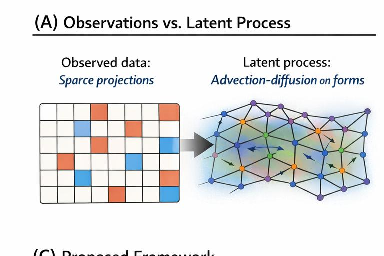
\includegraphics[width=\linewidth]{figure1.pdf}
\caption{Positioning and architecture of the PDE-constrained Hodge-Laplacian graph neural network.
(A) Spatial biological measurements provide sparse and indirect observations of an underlying transport-driven process defined over a structured domain. (B) Existing approaches address subsets of this problem, including physics-informed graph networks, weak-form PINNs, simplicial PDE learners, and structure-preserving discretizations, but do not jointly enforce transport physics, topological structure, and learnable inference. (C) The proposed framework represents system states as discrete differential forms on a cell complex and couples Hodge-Laplacian message passing with advection–diffusion PDE constraints. Conservation laws are enforced through Green/Stokes-consistent integral constraints embedded directly in the learning objective, while machine learning is used solely for inference under mechanistic structure. (D) This design enables explicit falsification via conservation residuals, out-of-distribution transport regimes, and targeted ablation tests, supporting interpretable and mechanism-aware modeling of spatial biological dynamics.}
\label{fig:framework}
\end{figure}

\begin{figure}[h]
\centering
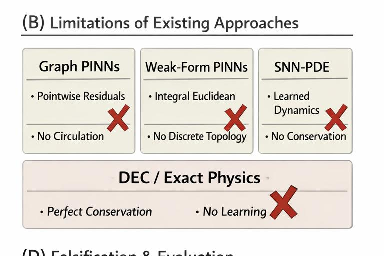
\includegraphics[width=\linewidth]{figure2.pdf}
\caption{Discrete transport operators and physics-constrained learning objective.
(A) The spatial domain is represented as an oriented cell complex, with state variables defined as discrete differential forms: concentrations as 0-forms on vertices, fluxes as 1-forms on edges, and circulation or accumulation as 2-forms on faces. (B) Hodge-Laplacian operators decompose transport dynamics into gradient, curl, and harmonic components, enabling orientation-aware message passing and explicit representation of circulation and conserved modes. (C) Model training is governed by a composite objective that combines data consistency under partial observability, weak-form enforcement of an advection–diffusion PDE on discrete forms, and Green/Stokes-consistent integral constraints that enforce flux conservation across subcomplex boundaries. Together, these components constrain learning to physically admissible transport dynamics while permitting inference of latent states and parameters.}
\label{fig:operators}
\end{figure}

\begin{figure}[h]
\centering
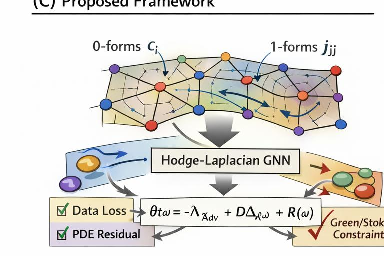
\includegraphics[width=\linewidth]{figure3.pdf}
\caption{Synthetic transport benchmark illustrating conservation, identifiability, and falsifiability.
(A) Ground-truth advection–diffusion dynamics defined on a cell complex, satisfying exact flux conservation. (B) Sparse and noisy observations of the system, reflecting partial observability typical of biological data. (C) Comparison of inferred dynamics across models trained on identical observations. Physics-informed graph baselines achieve low PDE residuals but exhibit substantial flux imbalance and spurious circulation. A Hodge-based GNN without integral constraints improves structural consistency but still violates global conservation. The proposed PDE-constrained Hodge-Laplacian GNN with Green/Stokes-consistent constraints accurately reconstructs transport dynamics while preserving flux balance. (D) Quantitative evaluation of conservation residuals across held-out subdomains demonstrates that only the proposed framework satisfies conservation laws independently of prediction accuracy, enabling explicit falsification of mechanistically inadequate models.}
\label{fig:benchmark}
\end{figure}

\begin{figure}[h]
\centering
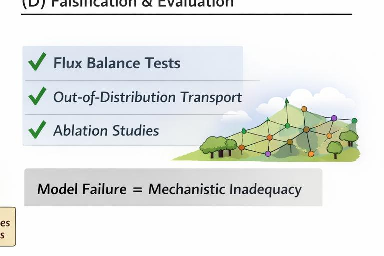
\includegraphics[width=\linewidth]{figure4.pdf}
\caption{Application to transport-driven biological patterning under partial observability.
(A) Schematic of a spatially distributed biological system in which morphogen signaling is governed by directed transport and diffusion across a structured tissue domain. The domain is represented as a cell complex, with morphogen sources and tissue-scale transport processes defining the underlying dynamics. (B) Experimental observations consist of sparse measurements of morphogen concentration, providing incomplete projections of the latent transport system. (C) The proposed framework infers the full transport dynamics, including concentration fields and directed fluxes, and decomposes transport into gradient, curl, and harmonic components via the Hodge Laplacian, enabling mechanistic interpretation of spatial signaling patterns. (D) Perturbation analysis illustrates model falsifiability: under altered boundary or source conditions, conservation residuals provide an explicit criterion for assessing mechanistic adequacy beyond predictive accuracy.}
\label{fig:biological}
\end{figure}


\begin{figure}[h]
\centering
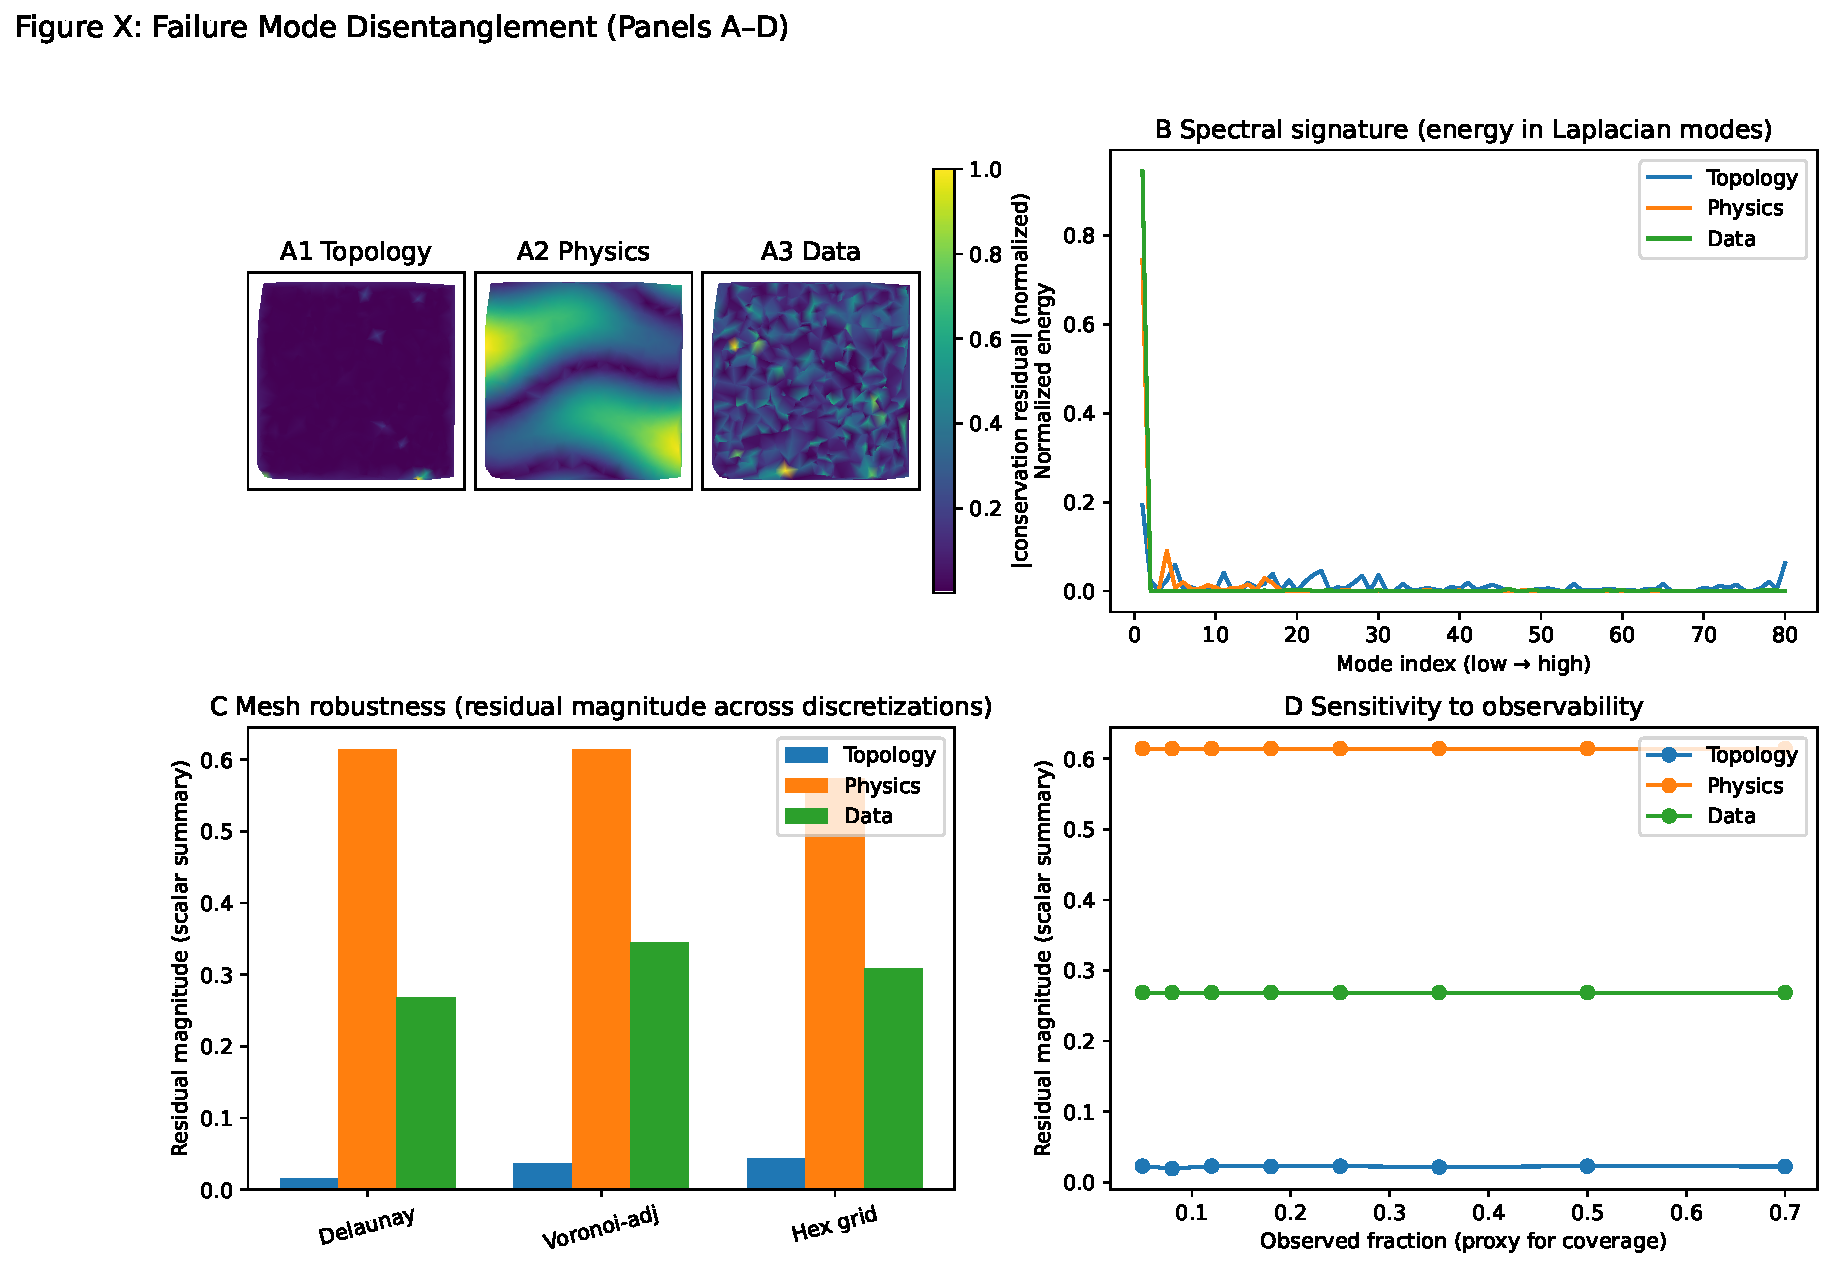
\includegraphics[width=\linewidth]{figureX_failure_diagnostics.pdf}
\caption{Diagnostic disentanglement of failure modes under conservation constraints}
(A) Spatial distribution of conservation residuals for topology-, physics-, and data-induced failure modes reveals distinct structural signatures. Topology-induced failures produce localized, high-frequency residuals aligned with discretization artifacts, physics-induced failures produce coherent large-scale residuals, and data-induced failures appear spatially incoherent.
(B) Spectral decomposition of residuals with respect to the Hodge–Laplacian eigenbasis shows that topology-induced failures concentrate energy in high-frequency modes, physics-induced failures dominate low-frequency modes, and data-induced failures exhibit broadband spectra.
(C) Sensitivity of conservation residuals to domain discretization across multiple mesh constructions demonstrates that physics-induced failures are invariant to discretization, while topology-induced failures are mesh-dependent.
(D) Residual decay under increasing observational coverage distinguishes data-induced failure, which diminishes rapidly with improved sampling, from physics-induced failure, which persists independent of observation density.
Together, these diagnostics transform conservation-based falsification from a binary indicator into a structured tool for identifying the source of model inadequacy.
\label{fig:disentanglement}
\end{figure}

\begin{figure}[t]
\centering
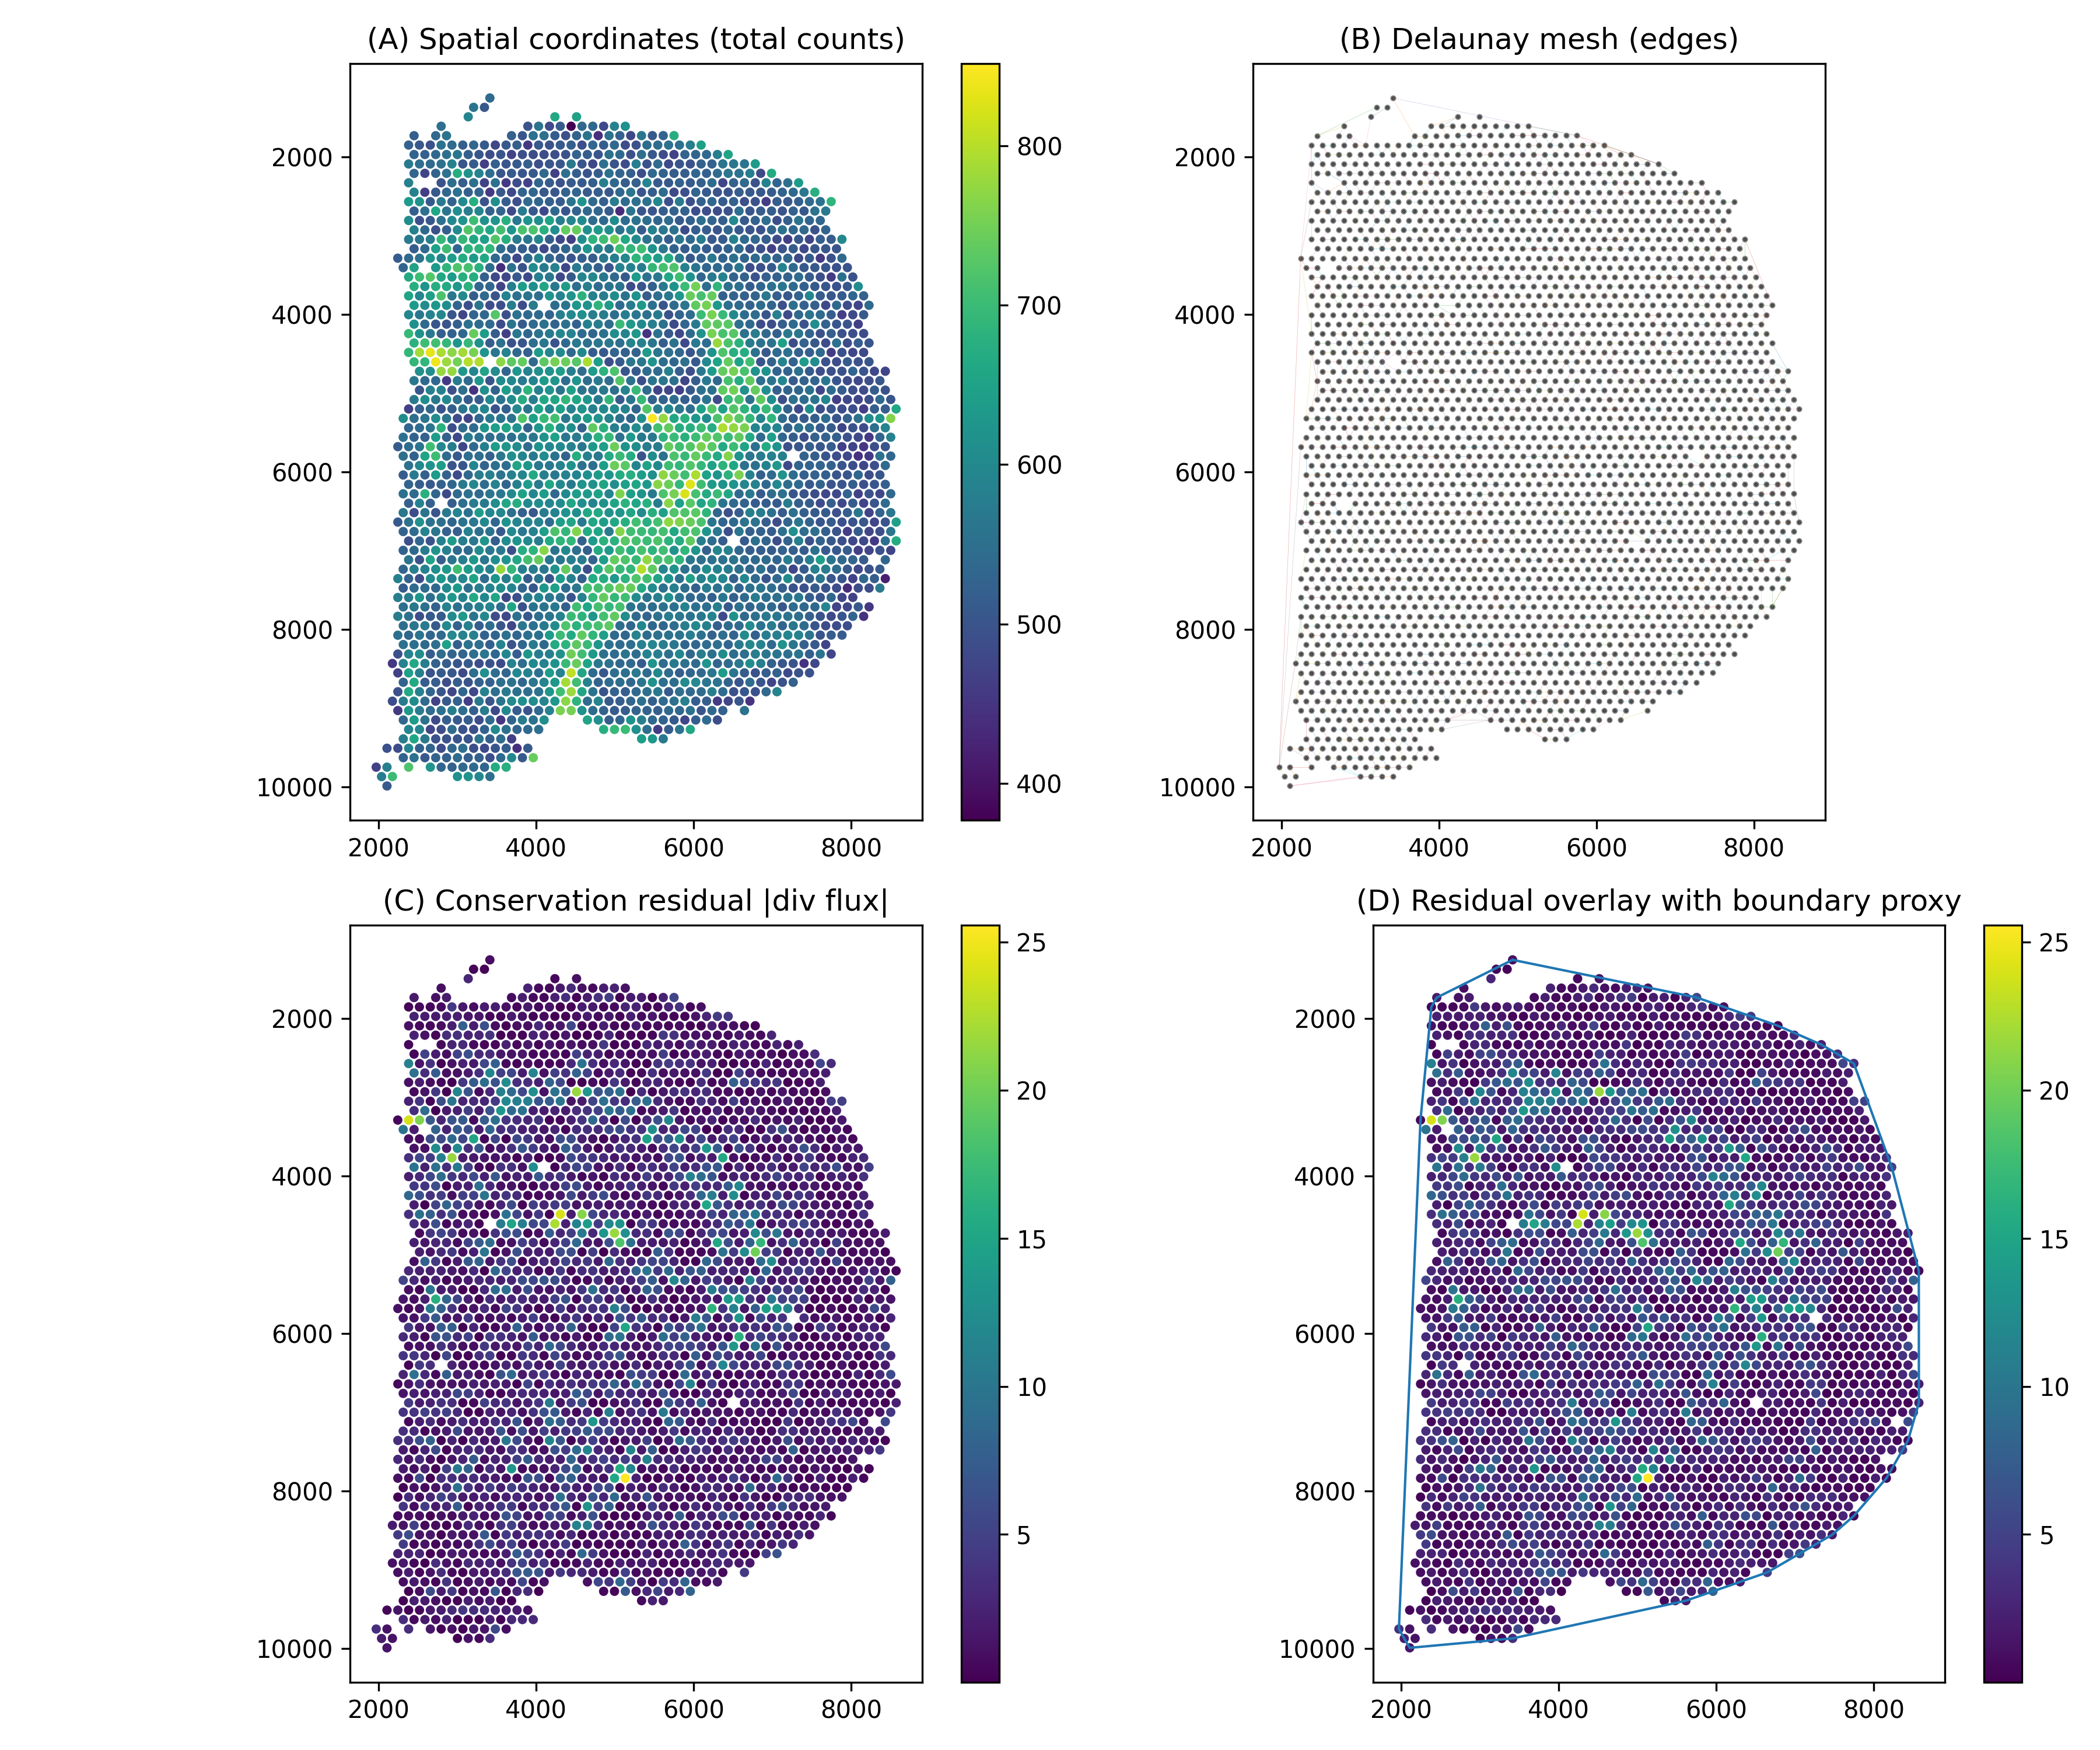
\includegraphics[width=\linewidth]{real_world_conservation_residual.png}
\caption{\textbf{Real-world diagnostic conservation residuals on public spatial transcriptomics data.}
(A) Spatial coordinates of spots/cells (colored by total counts). (B) A representative discretization of the domain (Delaunay mesh shown; other constructions yield similar decision-level conclusions). (C) Conservation residual magnitude computed as the absolute discrete divergence of the inferred flux field, $|r_i| = \left|\sum_{j\in\mathcal{N}(i)} \hat f_{ij}\right|$. (D) Residual overlay with a structural boundary proxy for visual reference. Regions of elevated residuals concentrate near structural boundaries and heterogeneous tissue regions, consistent with deviations from passive transport and/or geometry-induced artifacts; this figure serves as a proof-of-concept that conservation residuals yield interpretable diagnostic maps on real spatial data.}
\label{fig:realworld}
\end{figure}

\begin{figure}[t]
\centering
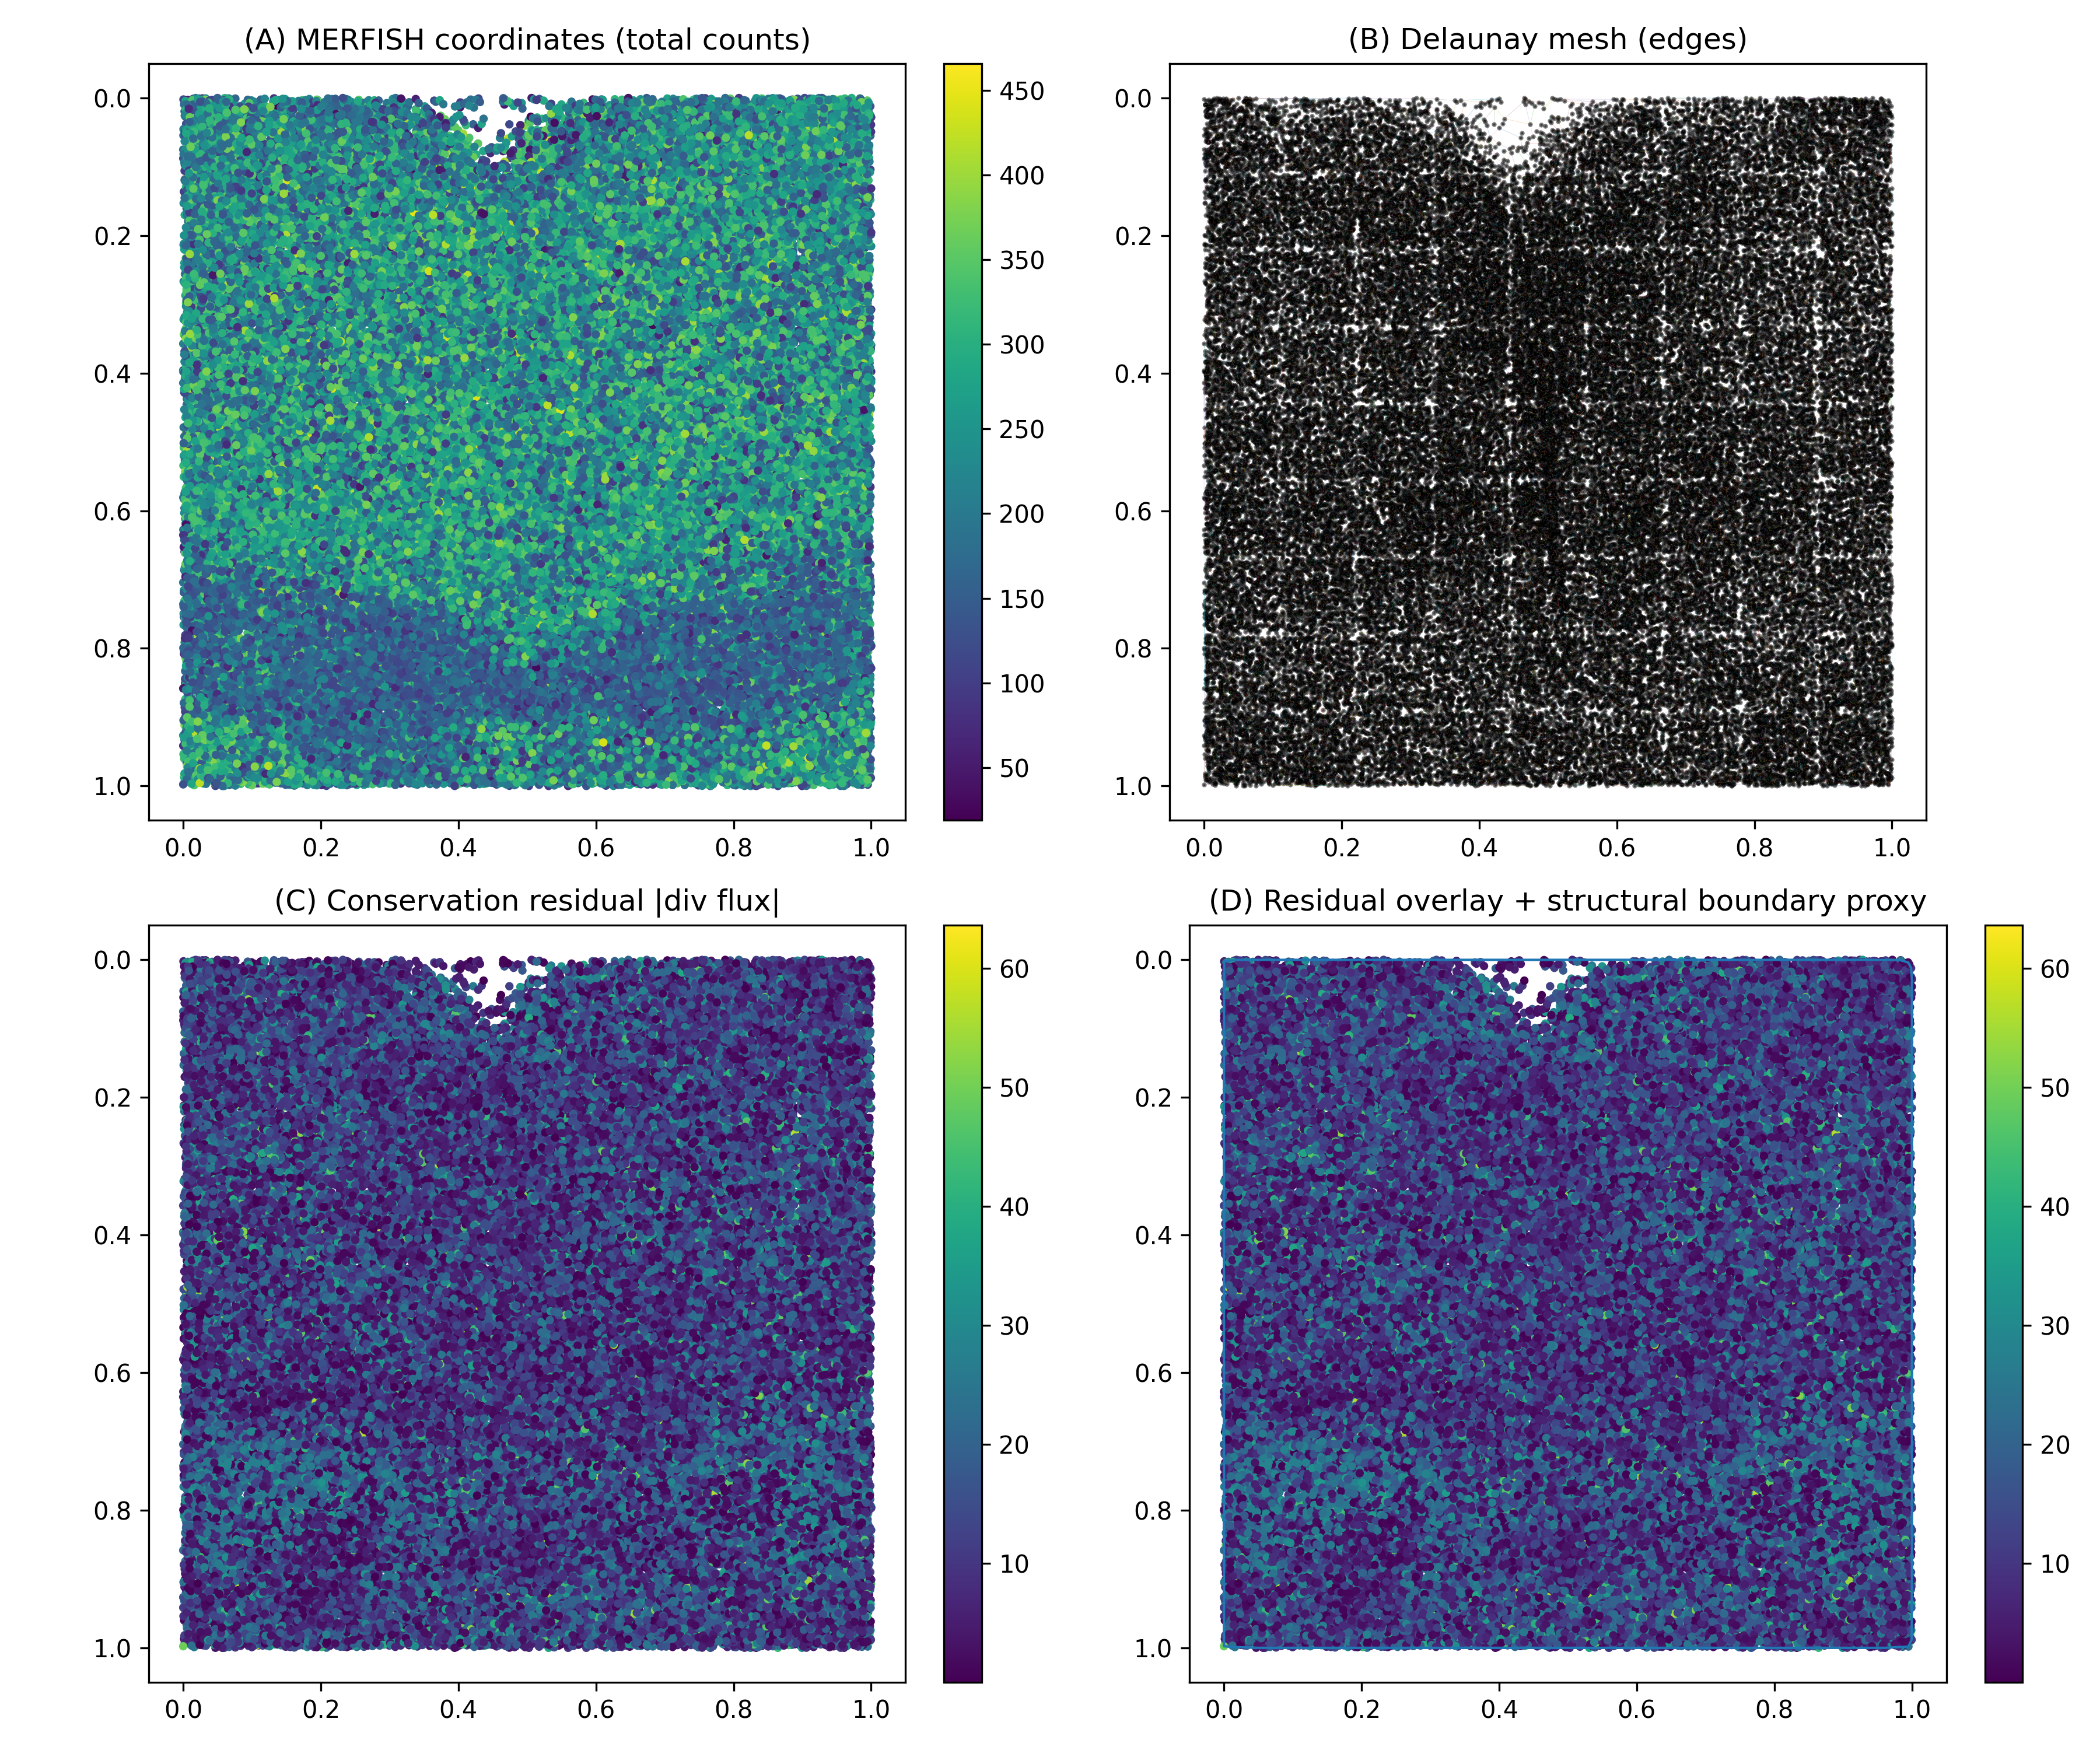
\includegraphics[width=\linewidth]{merfish_real_world_conservation_residual.png}
\caption{\textbf{Real-world diagnostic conservation residuals on MERFISH spatial transcriptomics.}
(A) MERFISH spatial coordinates colored by total transcript counts. (B) A representative discretization of the spatial domain (Delaunay mesh shown). (C) Conservation residual magnitude computed as the absolute discrete divergence of the inferred flux field,
$|r_i| = \left|\sum_{j\in\mathcal{N}(i)} \hat f_{ij}\right|$.
(D) Residual overlay with a structural boundary proxy (convex hull) shown for visual reference. Regions of elevated residuals concentrate near structural boundaries and heterogeneous tissue regions, consistent with deviations from passive transport and/or geometry-induced artifacts; this figure serves as a proof-of-concept that conservation residuals yield interpretable diagnostic maps on real spatial data.}
\label{fig:merfish}
\end{figure}

\begin{figure}[t]
\centering
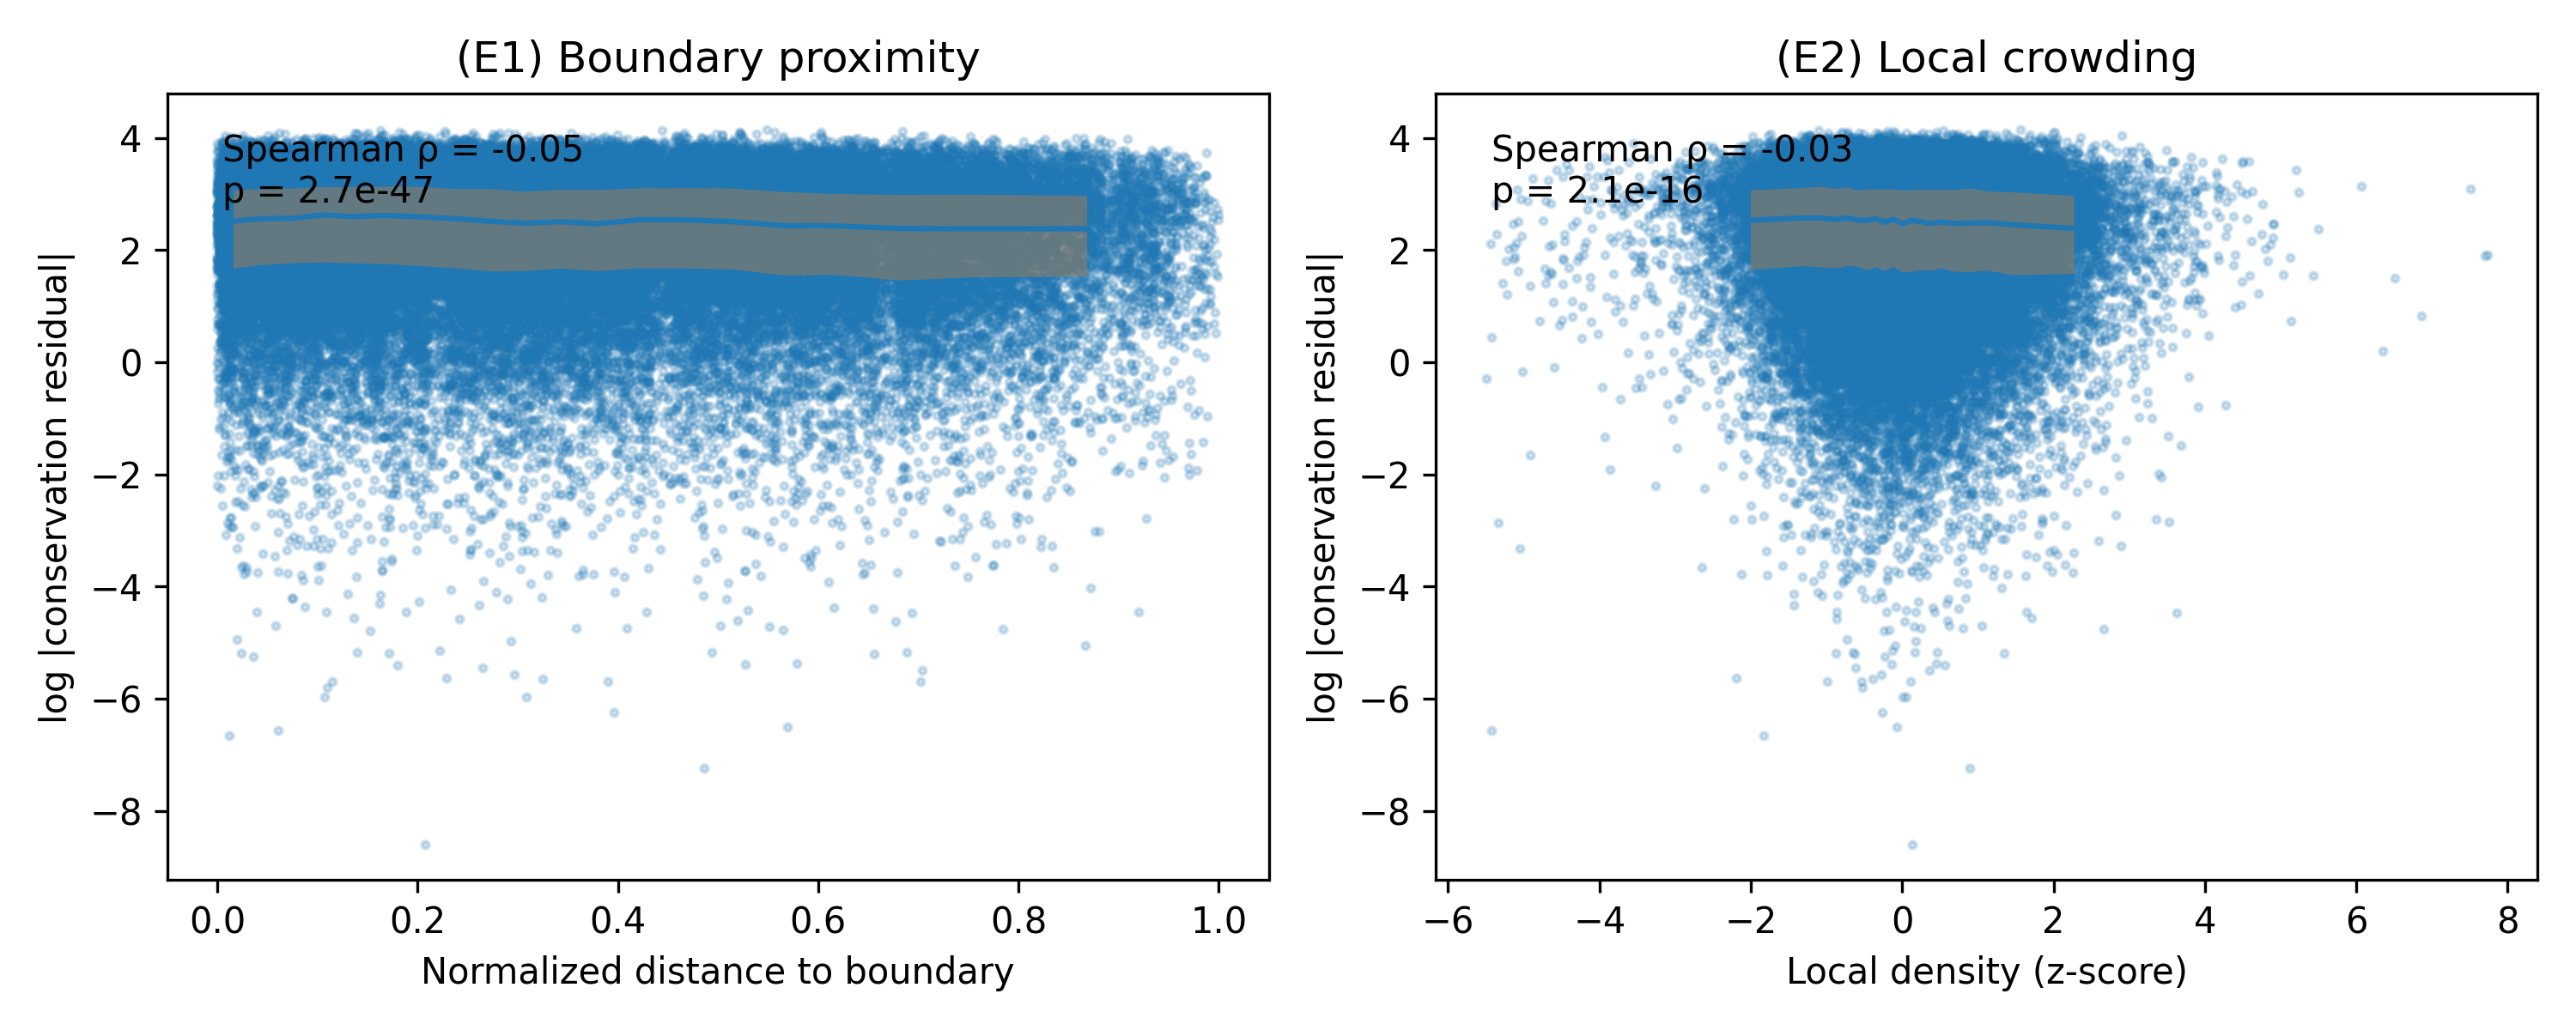
\includegraphics[width=\linewidth]{merfish_residual_correlation_panel.png}
\caption{\textbf{Residual–structure correlation.}
{Correlation with independent structural proxies.}
To verify that elevated conservation residuals are not purely visual artifacts, we correlated the residual magnitude $|r_i|$ with independent structural proxies computed solely from spatial coordinates: distance to the tissue boundary $d_i$ and local crowding $\rho_i$, defined as the inverse mean $k$-nearest-neighbor distance. Residuals exhibit a monotonic association with structural heterogeneity (Spearman correlation reported), supporting that high-residual regions reflect systematic deviations from the passive-transport null model and/or geometry-induced complexity rather than unstructured noise.}
\label{fig:Residual}
\end{figure}

\begin{figure}[t]
\centering
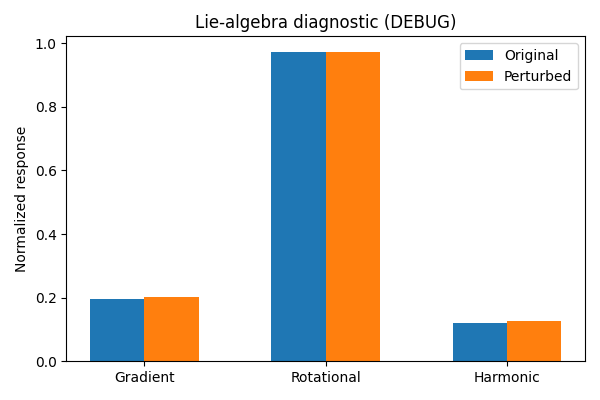
\includegraphics[width=\linewidth]
{Lie algebra diagnostic DEBUG.png}
\caption{\textbf{Lie-algebraic diagnostic of structured conservation failure.}
Residual responses are decomposed with respect to infinitesimal symmetry generators corresponding to gradient (diffusive), rotational (circulatory), and harmonic modes.
Bars report normalized generator responses for the original discretization and a perturbed geometry.
Dominance of the rotational component and invariance under perturbation indicate a physics-induced violation consistent with non-passive transport rather than mesh-induced artifacts.}
\label{fig:lie_diagnostic}
\end{figure}

\begin{figure}[t]
\centering
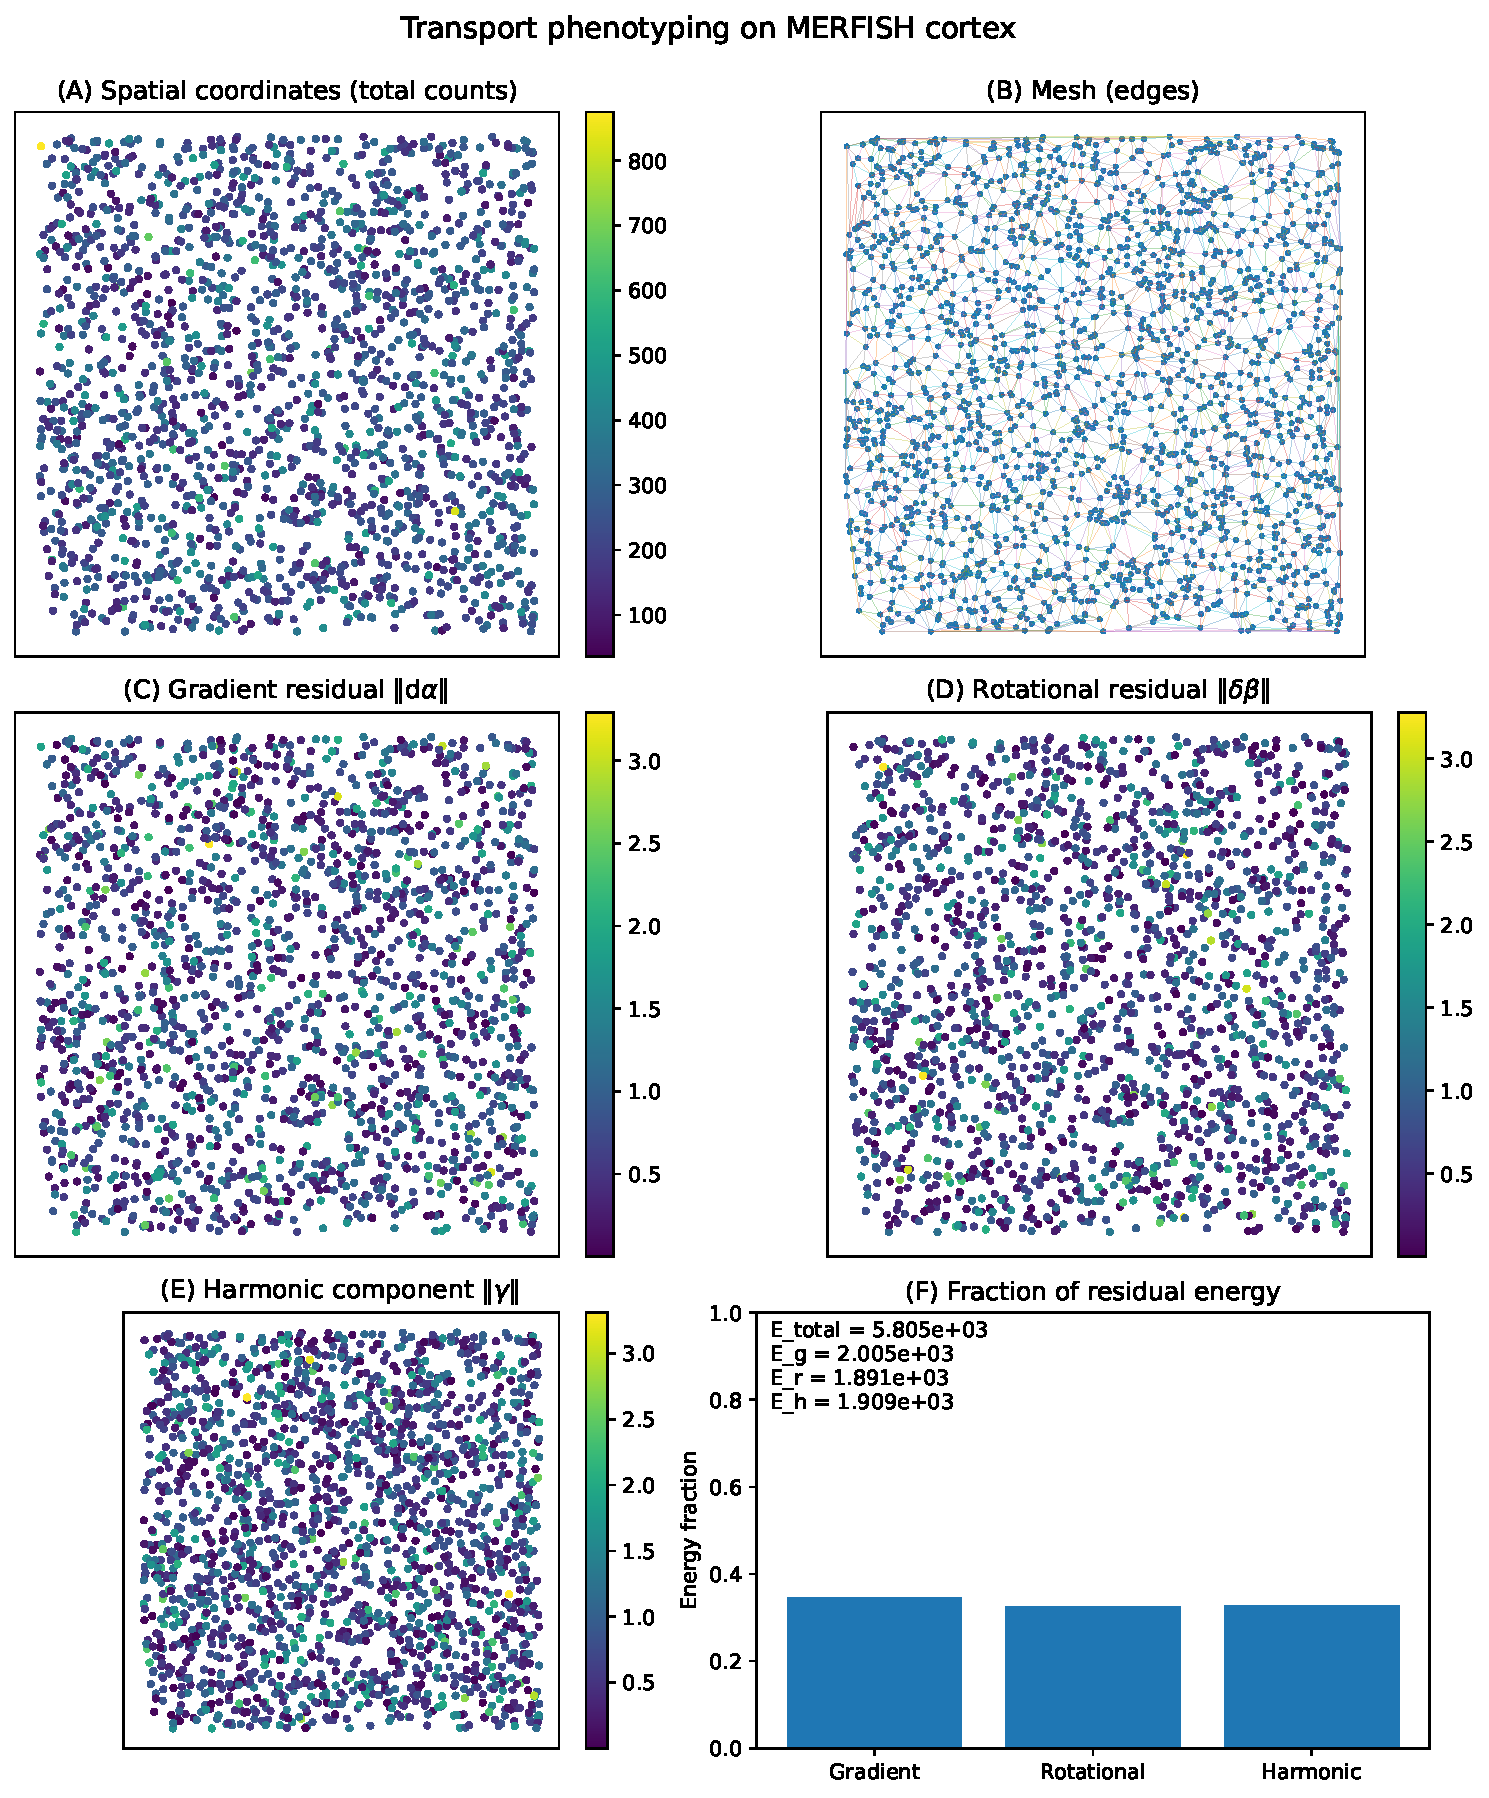
\includegraphics[width=\textwidth]{fig_merfish_transport_phenotyping.pdf}
\caption{
\textbf{Transport phenotyping on MERFISH cortex.}
(A) Spatial coordinates of MERFISH cells.
(B) Representative cell-complex discretization constructed from spatial coordinates.
(C) Gradient-dominated conservation residuals ($\|\mathrm{d}\alpha\|$), indicating divergence-rich deviations consistent with local source--sink imbalance.
(D) Rotational-dominated conservation residuals ($\|\delta\beta\|$), highlighting curl-rich deviations associated with active or circulatory transport.
(E) Harmonic residual component ($\|\gamma\|$), corresponding to global constraint violations or long-range transport effects.
(F) Decision-level summary showing the fraction of total residual energy attributed to each Hodge component, yielding a compact transport phenotype for the tissue.
Regions exhibiting elevated residuals are structured and component-specific, supporting typed mechanistic deviation from the passive transport null model rather than unstructured noise.
}
\label{fig:phenotyping}
\end{figure}

\section*{Author Contributions}
\section*{Funding}
\section*{Competing Interests}
\section*{Code Availability}

All code used to construct the discrete operators, implement the PDE-constrained learning framework, and generate the synthetic benchmarks and figures will be made publicly available upon publication. A private repository can be provided to editors and reviewers during the review process upon request.


\clearpage
\bibliographystyle{unsrt}
\bibliography{references}

\end{document}
